\subsection{Контрольная работа 1. Базовый поток. 30.10.2014}
\subsubsection*{Тест}

\begin{enumerate}

\item Если $A \cap B = \emptyset$, то $A$ и $B$ — независимые события. Да. Нет.

\item Попарно независимые события независимы в совокупности. Да. Нет.

\item $\P(A \cap B) \le \P(A|B)$. Да. Нет.

\item Для любого числа $a$ и любой случайной величины $X$: $\P(X=a)>0$. Да. Нет.

\item Любая неотрицательная функция $f(x)$, такая что $\int_{-\infty}^{+\infty} f(x) dx = 1$, может быть функцией плотности некоторой случайной величины. Да. Нет.

\item Функция распределения имеет не более, чем счетное, число точек разрыва. Да. Нет.

\item Для того, чтобы существовало математическое ожидание абсолютно непрерывной случайной величины достаточно, чтобы $\int_{-\infty}^{+\infty} x f(x) dx < \infty$. Да. Нет.

\item В Пуассоновском распределении математическое ожидание всегда совпадает с дисперсией.	Да. Нет.

\item Математическое ожидание суммы случайных величин всегда равно сумме их математических ожиданий.	Да. Нет.

\item Дисперсия суммы случайных величин всегда равна сумме их дисперсий.	Да. Нет.

\item Хорошо, что не было вопросов про корреляцию.	Да. Нет.

\end{enumerate}

\subsubsection*{Задачи}

\begin{enumerate}



\item Вася забыл какую-то (какую?) формулу. Он помнит, что она начинается с $\P(A|B) = $ . Дальше была дробь, три буквы $P$ со скобками после них и в сумме по две буквы $A$ и $B$ внутри этих скобок. Ещё там была вертикальная черта «|». Из этих элементов Вася случайным образом составляет формулу.
\begin{enumerate}
\item С какой вероятностью Вася напишет правильную формулу?
\item Напишите формулу, которую забыл Вася.
\end{enumerate}

Примечание: Вася всё-таки успел сходить на пару лекций по теории вероятностей и помнит, что $\P(A|B)$ и $\P(B|A)$ — это не одно и то же, «|» должна стоять именно между буквами (то ли $A|B$, то ли $B|A$), а в скобках, которые идут после $P$, должно хоть что-то стоять. При этом формула должна иметь смысл, то есть  $\P(A|B)$   не должна выражаться через себя же, и дробь не должна быть сократимой.

\item Точка с координатами $(\xi, \eta)$ бросается наудачу в треугольник с вершинами $(1,0)$, $(0,0)$, $(0,1)$.  Сформулируйте определение независимости двух событий и проверьте, будут ли события $A=\{ \xi < 1/2 \}$  и $B=\{ \eta < 1/2 \}$  независимыми?

\item На учениях три самолёта одновременно и независимо атакуют цель. Известно, что первый самолёт поражает цель с вероятностью $0.6$, второй — $0.4$, третий — $0.3$. При разборе учений выяснилось, что цель была поражена только одним самолётом. Какова вероятность того, что это был первый самолёт?

\item Книга в $500$ страниц содержит $400$ опечаток. Предположим, что каждая из них независимо от остальных опечаток может с одинаковой вероятностью оказаться на любой странице книги.
\begin{enumerate}

\item Определите вероятность того, что на $13$-й странице будет не менее двух опечаток, в явном виде и с помощью приближения Пуассона.
\item Определите наиболее вероятное число, математическое ожидание и дисперсию числа опечаток на $13$-ой странице.
\item Является ли $13$-ая страница более «несчастливой», чем все остальные (в том смысле, что на $13$-ой странице ожидается большее количество очепяток, чем на любой другой)?
\end{enumerate}

Подсказка.  Можно считать, что опечатки «выбирают» любую из страниц для своего появления независимо друг от друга. Успех заключается в выборе $13$-ой страницы. Вероятность успеха?

\item Вероятность того, что медицинский тест выявит наличие заболевания, когда оно действительно есть, называется чувствительностью теста. Специфичностью теста называется вероятность того, что тест покажет отсутствие заболевания, когда пациент здоров. Вероятность того, что пациент болен, когда тест показал наличие заболевания, называется прогностической силой теста. Предположим, что только 1\,\%  всего населения страдает данным заболеванием.  Чувствительность используемого теста равна $0.9$, а специфичность — $0.95$.
\begin{enumerate}
\item Какова вероятность того, что у случайно выбранного человека тест покажет наличие заболевания?
\item Какова прогностическая сила теста? Что нужно сделать, чтобы её повысить?
\end{enumerate}

\item Функция плотности случайной величины $X$ имеет вид:
\begin{equation*}
f(x) =
 \begin{cases}
   1.5 (x-a)^2 &, x \in [0,a]\\
   1.5 (x+a)^2 &, x \in [-a,0]\\
   0 &, x \not\in [-a,a]
 \end{cases}
\end{equation*}

\begin{enumerate}
\item Найдите константу $a$, вероятность попадания в отрезок $\left[1/2, 2 \right]$, математическое ожидание $X$ и дисперсию случайной величины $X$.
\item Нарисуйте функцию распределения случайной величины $X$.
\end{enumerate}

\item Вася случайным образом посещает лекции по ОВП (Очень Важному Предмету). С вероятностью $0.9$ произвольно выбранная лекция полезна, и с вероятностью $0.7$ она интересна. Полезность и интересность — независимые друг от друга и от номера лекции свойства. Всего Вася прослушал 30 лекций.
\begin{enumerate}
\item Определите математическое ожидание и дисперсию числа полезных лекций и числа интересных лекций, прослушанных Васей.
\item Определите математическое ожидание числа бесполезных и неинтересных лекций, прослушанных Васей, и числа лекций, обладающих хотя бы одним из свойств (полезность,  интересность).
\end{enumerate}

\item Пусть $\E(X) = 1$, $\E(Y) = 2$, $\E(X^2) = 5$, $\E(XY) = -1$. Найдите:
\begin{enumerate}
\item $\E(2X + Y - 4)$
\item $\Var(X)$, $\Var(Y)$
\item $\Cov(X,Y)$, $\Corr(X,Y)$
\item $\Var(X-Y-1)$,  $\Var(X+Y+1)$
\item $\Cov(X-Y-1, X+Y+1)$,  $\Corr(X-Y-1, X+Y+1)$
\end{enumerate}

\item Совместное распределение случайных величин $X$ и $Y$ задано в виде таблицы:

\begin{tabular}{c|cc}
\toprule
 & $X=1$ & $X=2$ \\ \midrule
$Y=-1$ & $0.1$ & $0.2$ \\
$Y=0$ & $0.2$ & $0.3$ \\
$Y=1$ & $0$ & $0.2$ \\ \bottomrule
\end{tabular}

\begin{enumerate}
\item Найти частные распределения $Y$ и $Y^2$
\item Найти ковариацию случайных величин $X$ и $Y$
\item Можно ли утверждать, что случайные величины зависимы?
\end{enumerate}

\item Бонусная задача

Какова вероятность того, что наугад выбранный ответ на этот вопрос окажется верным (искомую вероятность вычислить и записать!)?
\begin{enumerate}
\item 0.25
\item 0.5
\item 0.6
\item 0.25
\end{enumerate}

\end{enumerate}

\subsection{Решение кр 1. Базовый поток}
\begin{enumerate}
\item Внимательно читайте примечание! Всего 6 возможных ситуаций, только 1 — благоприятная. Требуемая вероятность равна $1/6$.

\item
Два события $A$ и $B$ независимы, если: $\P(AB) = \P(A) \P(B)$.

Проверим, независимы ли события $A = \{ \xi < 1/2 \} $ и  $B = \{ \eta < 1/2 \} $:

$\P(AB)$ ищется как отношение площади квадрата с вершинами в $(0,\,0)$; $(0,\,1/2)$; $(1/2,\,1/2)$; $(1/2,\,0)$ к площади данного треугольника, т.е.:
\[\P(AB) = \frac{(1/2)^2}{1/2}= \frac{1}{2}\]

$\P(A)$ ищется как отношение площади трапеции с вершинами в $(0,\,0)$; $(0,\,1)$; $(1/2,\,1/2)$; $(1/2,\,0)$ к площади данного треугольника, т.е.:
\[\P(A) = \frac{(1/2)\cdot (3/2) \cdot (1/2)}{1/2}= \frac{3}{4}\]

$\P(B)$ ищется как отношение площади трапеции с вершинами в $(0,\,0)$; $(1,\,0)$; $(1/2,\,1/2)$; $(0,\,1/2)$ к площади данного треугольника, т.е.:
\[\P(B) = \frac{(1/2)\cdot (3/2) \cdot (1/2)}{1/2}= \frac{3}{4}\]

\[\P(A)\cdot \P(B) = \frac{3}{4} \cdot  \frac{3}{4} = \frac{9}{16} \ne \frac{1}{2} = \P(AB)\]

Итак, события $A$ и $B$ зависимы.

\item
Пусть событие $A$ = \{ Цель была поражена первым самолетом \}, событие $B$ = \{ Цель была поражена только одним самолетом \}. Тогда событие $AB$ = \{Первый самолет поразил цель, второй и третий — промахнулись  \}. По формуле условной вероятности:

\[\P(A|B) = \frac{\P(AB)}{\P(B)} = \frac{0.6 \cdot 0.6 \cdot 0.7}{0.6\cdot 0.6 \cdot 0.7 + 0.4 \cdot 0.4 \cdot 0.7 + 0.4 \cdot 0.6 \cdot 0.3} = \frac{0.252}{0.436} \approx 0.578\]

\item
Удобно рассуждать следующим образом: предположим, что каждая опечатка наугад (\textcolor{red}{с равными вероятностями и независимо от других опечаток}) выбирает, на какую страницу ей попасть.


\begin{enumerate}
\item Пусть $X$ - число опечаток на 13 странице. \[\P(X \geqslant 2) = 1 - \P(X=0) - \P(X=1) \]
$\P(X=0) = \left( \frac{499}{500} \right)^{400}$ — каждая из 400 опечаток не должна попасть на 13 страницу.\\
$\P(X=1) = 400\cdot\frac{1}{500}\cdot\left( \frac{499}{500} \right)^{399}$ — ровно одна опечатка (а есть 400 вариантов) должна попасть на 13 страницу, а остальные — мимо. Соответственно:
\[
\P(X \geqslant 2) = 1 - \left( \frac{499}{500} \right)^{400} - 400\cdot\frac{1}{500}\cdot\left( \frac{499}{500} \right)^{399} \approx 0.1911357
\]
Это если считать в явном виде. А если пользоваться приближением Пуассона:
\[
p(k) = \P(X = k) = \frac{\lambda^k}{k!}e^{-\lambda}
\]
неплохо бы вспомнить, что параметр $\lambda$ это математическое ожидание $X$, поэтому расчеты здесь пока оставим до лучших времен.

\item Пусть $X$ - число опечаток на 13 странице. Введем случайную величину
\[X_i =
\begin{cases}
1 & \text{если } i\text{-ая опечатка попала на 13 страницу}\\
0 & \text{если нет}
\end{cases}
\]
Тогда $X = \sum\limits_{i=1}^{400}X_i$. Рассмотрим отдельно $X_i$:

\begin{tabular}{@{}ccc@{}}
\toprule
$X$         & $1$             & $0$               \\ \midrule
$\P(\cdot)$ & $\frac{1}{500}$ & $\frac{499}{500}$ \\ \bottomrule
\end{tabular}

Так как $i$-ая опечатка наугад выбирает одну страницу из 500 и это должна быть именно 13.

Тогда:
\[
\E(X_i) = \frac{1}{500} = \E(X^2_i) \Rightarrow
\]
\[
\Rightarrow \Var(X_i) = \E(X^2_i) - (\E(X_i))^2 = \frac{1}{500} - \left(\frac{1}{500}\right)^2 = \frac{499}{500^2}
\]
Значит
\[
\E(X) = \E\left(\sum\limits_{i=1}^{400}X_i\right) = \sum\limits_{i=1}^{400}\E(X_i)  = \frac{400}{500} = 0.8
\]

\[
\Var(X) = \Var\left(\sum\limits_{i=1}^{400}X_i\right) = \sum\limits_{i=1}^{400}\Var(X_i) = 400\cdot\frac{499}{500^2} = 0.8\cdot\frac{499}{500}
\]

Теперь мы знаем, что $\lambda = \E(X) = 0.8$ поэтому можем вернуться к пункту (а):
\[
\P(X \geqslant 2) = 1 - \P(X=0) - \P(X=1)  = 1 - \frac{0.8^0}{0!}e^{-0.8} - \frac{0.8^1}{1!}e^{-0.8} = 0.1912079
\] \vspace{-1.2cm}

\hspace{13cm} \fcolorbox{ForestGreen}{white}{So close!}

Осталось найти наиболее вероятное число опечаток на 13 странице:
\[
\P(X=k) = \frac{0.8^k}{k!}e^{-0.8} \rightarrow \max \limits_k
\]
Очевидно, что эта функция убывает по $k$, ведь с ростом $k$:\\
 $k!$ растет, а $0.8^k$ убывает. Значит наиболее вероятное число ошибок — $X = 0$


\item \href{https://en.wikipedia.org/wiki/Triskaidekaphobia}{Ох уж эти предрассудки!} 13-я страница точно такая же как и все остальные, ведь везде в решении можно просто заменить номер 13 на любой другой и ничего не изменится.

\end{enumerate}

\item
Перепишем условие задачи:

Чувствительность теста = \\$=\P(\text{Медицинский тест показывает наличие заболевания} | \text{Заболевание есть})$

Специфичность теста = \\$=\P(\text{Медицинский тест показывает отсутствие заболевания} | \text{Заболевания нет})$

Прогностическая сила теста = \\$=\P(\text{Заболевание есть} | \text{Медицинский тест показывает наличие заболевания})$

$\P(\text{Заболевание есть}) = 0.01 \Rightarrow \P(\text{Заболевания нет}) = 0.99 $

По условию чувствительность теста равна 0.9, тогда из формулы условной вероятности:

\[\P(\text{Мед. тест пок-ет наличие заб-ия} | \text{Заб-ие есть}) = \]
\[\frac{\P(\text{Мед. тест пок-ет наличие заб-ия, Заб-ие есть})}{\P(\text{Заб-ие есть})} \Rightarrow\]
\[\Rightarrow \P(\text{Мед. тест пок-ет наличие заб-ия, Заб-ие есть}) = 0.9 \cdot 0.01 = 0.009\]

При этом очевидно, что:
\[\P(\text{Заболевание есть}) = \P(\text{Мед. тест пок-ет наличие заб-ия, Заб-ие есть}) + \]
\[+ \P(\text{Мед. тест пок-ет отсутствие заб-ия, Заб-ие есть}) \Rightarrow\]
\[\Rightarrow \P(\text{Мед. тест пок-ет отсутствие заб-ия, Заб-ие есть}) = 0.01 - 0.009 = 0.001\]

По условию специфичность теста равна 0.95, тогда из формулы условной вероятности:
\[\P(\text{Мед. тест пок-ет отсутствие заб-ия} | \text{Заб-ия нет}) = \]
\[\frac{\P(\text{Мед. тест пок-ет отсутствие заб-ия, Заб-ия нет})}{\P(\text{Заб-ия нет})} \Rightarrow\]
\[\P(\text{Мед. тест пок-ет отсутствие заб-ия, Заб-ия нет}) =0.95 \cdot 0.99 = 0.9405\]

При этом очевидно, что:
\[\P(\text{Заб-ия нет}) = \P(\text{Мед. тест пок-ет наличие заб-ия, Заб-ия нет}) + \]
\[+ \P(\text{Мед. тест пок-ет отсутствие заб-ия, Заб-ия нет}) \Rightarrow\]
\[\Rightarrow \P(\text{Мед. тест пок-ет наличие заб-ия, Заб-ия нет}) = 0.99 - 0.9405 = 0.0495\]

Теперь мы готовы отвечать на заданные вопросы:

\begin{itemize}
\item
\[\P(\text{Мед. тест пок-ет наличие заб-ия}) = \]
\[= \P(\text{Мед. тест пок-ет наличие заб-ия, Заб-ия нет}) + \]
\[+ \P(\text{Мед. тест пок-ет наличие заб-ия, Заб-ие есть}) = 0.009+0.0495 = 0.0585 \]

\item Прогностическая сила теста:

\[\P(\text{Заболевание есть} | \text{Медицинский тест показывает наличие заболевания}) = \]
\[= \frac{\P(\text{Мед. тест пок-ет наличие заб-ия, Заб-ие есть})}{\P(\text{Мед. тест пок-ет наличие заб-ия}) } = \frac{0.009}{0.0585} \approx 0.154\]

Для того, чтобы повысить прогностическую силу теста, необходимо понизить $\P(\text{Мед. тест пок-ет наличие заб-ия, Заб-ия нет}) $, а для этого необходимо повысить специфичность теста.

\end{itemize}

\item
\begin{itemize}
\item
Должно выполняться условие нормировки:
\[\int \limits_{-a}^0 1.5(x+a)^2 dx + \int \limits_0^a 1.5(x- a)^2  dx = 1   \]
\[0.5(x+a)^3 |_{-a}^0 + 0.5(x- a)^3 |_0^a  = 1   \]
\[0.5a^3 + 0.5a^3 = 1\]
\[a = 1\]

Теперь легко понять, как выглядит функция распределения (смотри определение функции распределения):

$F(x) = \begin{cases}
0, & x < 1 \\
0.5 (x+1)^3, & -1 \leqslant x <0 \\
1 + 0.5 (x-1)^3, & 0 \leqslant x < 1 \\
1, & x \geqslant 1
\end{cases}$

\[P\left(X \in \left[\frac{1}{2}, 2 \right]  \right) = F(2) - F\left(\frac{1}{2} \right) = 1 - 1 +0.5^4 = 0.5^4 \]

\[\E(X) = \int \limits_{-1}^0 x \cdot 1.5 (x + 1)^2 dx +  \int \limits_0^1 x \cdot 1.5 (x - 1)^2 dx = \]
\[= 1.5 \int \limits_{-1}^0\left( x^3 + 2x^2 + x\right) dx + 1.5 \int \limits_0^1\left( x^3 -2x^2 + x\right) dx = \]
\[=  \frac{3}{8} x^4 |_{-1}^0 + x^3 |_{-1}^0 + \frac{3}{4} x^2|_{-1}^0+    \frac{3}{8} x^4 |_0^1   - x^3 |_0^1 + \frac{3}{4} x^2|_0^1  = - \frac{3}{8}  + 1- \frac{3}{4} + \frac{3}{8} - 1 +\frac{3}{4} = 0 \]

А можно было заметить, что функция плотности — четная функция, поэтому сразу $\E(X) = 0$

Вычислим $\E(X^2)$:
\[\E(X^2) = \int \limits_{-1}^0 x^2 \cdot 1.5 (x + 1)^2 dx +  \int \limits_0^1 x^2 \cdot 1.5 (x - 1)^2 dx = \]
\[= 1.5 \int \limits_{-1}^0\left( x^4 + 2x^3 + x^2\right) dx + 1.5 \int \limits_0^1\left( x^4 -2x^3 + x^2\right) dx = \]
\[=  \frac{3}{10} x^5 |_{-1}^0 + \frac{3}{4} x^4|_{-1}^0 + \frac{1}{2} x^3 |_{-1}^0 +  \frac{3}{10} x^5 |_0^1 - \frac{3}{4} x^4|_0^1  + \frac{1}{2} x^3 |_0^1 =  \frac{1}{10}\]

\[\Var(X) = \E(X^2) - (\E(X))^2 = 0.1\]

\item Верим, что график $F(x)$, выписанной выше, вы построить можете :)
\end{itemize}
\item
Пусть $A = \{\text{«Лекция полезна»}\}$, $B = \{\text{«Лекция интересна»}\}$. Заметим, что лекции вообще независимы друг от друга.

\begin{enumerate}
\item Пусть $X_A$ — число полезных лекций, прослушанных Васей,  $X_B$ — число интересных лекций, прослушанных Васей. Введем случайную величину:
\[X_i =
\begin{cases}
1 & \text{если } i\text{-ая лекция была полезна}\\
0 & \text{если нет}
\end{cases}
\]

Тогда $X_A = \sum\limits_{i=1}^{30}X_i$. Рассмотрим отдельно $X_i$:

\begin{tabular}{@{}ccc@{}}
\toprule
$X$         & $1$             & $0$               \\ \midrule
$\P(\cdot)$ & $0.9$ & $0.1$ \\ \bottomrule
\end{tabular}

Вероятность 0.9 дана. Тогда:
\[
\E(X_i) = 0.9 = \E(X^2_i) \Rightarrow
\]
\[
\Rightarrow \Var(X_i) = \E(X^2_i) - (\E(X_i))^2 = 0.9 - 0.9^2 = 0.09
\]

Значит
\[
\E(X_A) = \E\left()\sum\limits_{i=1}^{30}X_i\right) = \sum\limits_{i=1}^{30}\E(X_i)  = 0.9\cdot30 = 27
\]
\[
\Var(X_A) = \Var\left(\sum\limits_{i=1}^{30}X_i\right) = \sum\limits_{i=1}^{30}\Var(X_i) = 0.09\cdot30 = 2.7
\]

Аналогично для числа интересных лекций можем получить:
\[
\E(X_B) = 0.7\cdot 30 = 21
\]
\[
\Var(X_A) = 0.21\cdot 30 = 6.3
\]


\item Так как интересность и полезность — независимые свойства лекций, то:\\
 $\P(\overline{A} \cap \overline{B}) = \P(\overline{A})\cdot \P(\overline{B}) = 0.3\cdot0.1 = 0.03$, где $\overline{A}$ значит «не $A$». В свою очередь:\\
 $\P(A\cup B) = \P(A\cap\overline{B}) + \P(B\cap\overline{A}) + \P(A\cap B) = 1 - \P(\overline{A})\cdot \P(\overline{B}) = 0.97$ , где $(A\cup B)$ значит «$A$ или $B$», а $(A\cap)B$ — «$A$ и $B$». Аналогично, путем введения бинарной случайной величины можем получить:
 \[
 \E(X_{\overline{A} \cap \overline{B}}) = 0.03 \cdot  30 = 0.9
 \]
 \[
 \E(X_{A\cup B}) = 0.97\cdot30 = 29.1
\]

\end{enumerate}

\item
Дано: $\E(X) = 1$, $\E(Y) = 2$, $\E(X^2) = 5$, $\E(Y^2) = 8$, $\E(XY) = -1$.

Будем использовать только свойства математического ожидания, ковариации и дисперсии, и ничего больше. Ни-че-го.

\begin{itemize}
\item  $\E(2X + Y - 4) = 2\E(X) + \E(Y) + \E(-4) = 2 + 2 - 4 = 0 $
\item $\Var(X) = \E(X^2) - (\E(X))^2 = 5 - 1 = 4 $
\item $\Var(Y) = \E(Y^2) - (\E(Y))^2 = 8 - 4 = 4 $
\item $\Cov(X, Y) = \E(XY) - \E(X)\E(Y) = -1 - 2 = -3$
\item $\Corr(X, Y) = \frac{\Cov(X, Y)}{\sqrt{\Var(X)}\sqrt{\Var(Y)}} = -\frac{3}{2\cdot 2} = -0.75$
\item $\Var(X-Y-1) = \Var(X) + \Var(Y) - 2\Cov(X, Y) = 4+4 -2(-3) = 14$
\item $\Var(X+Y+1) = \Var(X) + \Var(Y) + 2\Cov(X, Y) = 4+4+2(-3) =2 $
\item \begin{multline}
\Cov(X-Y-1, X+Y+1)=\E((X-Y)(X+Y))-\E(X-Y)\E(X+Y) = \\
\E(X^2-Y^2) - (\E(X)-\E(Y))(\E(X) + \E(Y)) =
\E(X^2) - \E(Y^2) - ((\E(X))^2 -(\E(Y))^2)=\\
 = \Var(X)-\Var(Y) = 0
 \end{multline}
 \item $\Cov(X-Y-1, X+Y+1)=0 \Rightarrow \Corr(X-Y-1, X+Y+1) = 0 $
\end{itemize}

\item Найдем частные распределения $Y$ и $Y^2$:
\begin{center}
\begin{tabular}{c|cc|c}
\toprule
 & $X=1$ & $X=2$ & $\sum$ \\ \midrule
$Y=-1$ & $0.1$ & $0.2$ & $0.3$ \\
$Y=0$ & $0.2$ & $0.3$ & $0.5$ \\
$Y=1$ & $0$ & $0.2$ & $0.2$ \\
$\sum$ & $0.3$ & $0.7$ & \\ \bottomrule
\end{tabular}
\end{center}

\begin{center}
\begin{tabular}{@{}cccc@{}}
\toprule
$Y$         & $-1$             & $0$      & $1$         \\ \midrule
$\P(\cdot)$ & $0.3$ & $0.5$  & $0.2$\\ \bottomrule
\end{tabular}
\end{center}

Так как $Y^2$ может принимать только значения 0 или 1:

\begin{center}
\begin{tabular}{@{}ccc@{}}
\toprule
$Y^2$         & $0$             & $1$               \\ \midrule
$\P(\cdot)$ & $0.5$ & $0.5$ \\ \bottomrule
\end{tabular}
\end{center}
А ковариация:
 \begin{multline*}
 \Cov(X, Y) = \E(XY) - \E(X)\E(Y) =
 ((-1)\cdot 1\cdot0.1 + (-1)\cdot2 \cdot 0.2 + 1\cdot2\cdot 0.2) -\\
 - (0.3\cdot1 + 0.7 \cdot 2)\cdot(0.3\cdot(-1) + 0.1\cdot 0.2) = 0.07
\end{multline*}

Так как $\Cov(X, Y) \ne 0$ — величины зависимы

\item Бонусная задача

Предположим, что правильный ответ 0.25. Но это невозможно, потому что вариантов ответа 0.25 — два (1 и 4), значит ответ 0.5 тоже был бы правильный. Предположим, что правильный 0.5. Тогда 0.25 тоже правильный — таких вариантов два из четырех, значит вероятность попасть в 0.25, выбрав ответ наугад, равна 0.5. Ответ 0.6, очевидно, неверен, потому что вероятность попасть в него равна 0.25. \\
\textbf{Правильный ответ:} 0
\end{enumerate}


\subsection{Праздник номер 1, i-поток, 30.10.2014}

\subsubsection*{ Часть 1}

\begin{enumerate}
%\item Винни-Пух собирается играть в Пустяки и готовит для игры палочки. Он нашел палку длиной 1 м, а дальше поступает следующим образом. Разламывает палку равномерно в случайном месте, одну полученную часть использует для игры, а вторую снова случайным образом делит на две части. Далее одну новую часть Винни-Пух снова использует для игры, а вторую новую часть снова делит на две. И так далее. Обозначим $X_i$ — длину палочки, использованной Винни-Пухом в $i$-ых Пустяках.

%Найдите функцию плотности $X_i$, $\E(X_i)$, $\Var(X_i)$

\item Вася купил два арбуза у торговки тети Маши и один арбуз у торговки тети Оли. Арбузы у тети Маши спелые с вероятностью 90\% (независимо друг от друга), арбузы у тети Оли спелые с вероятностью 70\%.

\begin{enumerate}
\item Какова вероятность того, что все Васины арбузы спелые?
\item Придя домой Вася выбрал случайным образом один из трех арбузов и разрезал его. Какова вероятность того, что это арбуз от тёти Маши, если он оказался спелым?
\item Какова вероятность того, что второй и третий съеденные Васей арбузы были от тёти Маши, если все три арбуза оказались спелыми?
\end{enumerate}


\item В большой большой стране живет очень большое количество $n»0$ семей. Количества детей в разных семьях независимы. Количество детей в каждой семье — случайная величина с распределением заданным табличкой:

\begin{tabular}{ccccc}
\toprule
$X$ & $0$ & $1$ & $2$ & $3$ \\ \midrule
$\P(\cdot)$ & $0.1$ & $0.3$ & $0.2$ & $0.4$ \\ \bottomrule
\end{tabular}

\begin{enumerate}
\item Исследователь Афанасий выбирает одну семью из всех семей наугад, пусть $X$ — число детей в этой семье. Найдите $\E(X)$ и $\Var(X)$.
\item Исследователь Бенедикт выбирает одного ребенка из всех детей наугад, пусть $Y$ — число детей в семье этого ребёнка. Как распределена величина $Y$? Что больше, $\E(Y)$ или $\E(X)$?
\end{enumerate}

\item Функция плотности случайной величины $X$ имеет вид
\[
f(x)=
\begin{cases}
\frac{3}{8} x^2, \text{ если } x\in [0;2] \\
0, \text{ иначе }
\end{cases}
\]
\begin{enumerate}
\item Не производя вычислений найдите $\int_{-\infty}^{+\infty}f(x)\,dx$
\item Найдите $\E(X)$, $\E(X^2)$ и дисперсию $\Var(X)$
\item Найдите $\P(X>1.5)$, $\P(X>1.5 \mid X>1)$
\item При каком $c$ функция $g(x)=c x f(x)$ будет функцией плотности некоторой случайной величины?
\end{enumerate}

\item Известно, что  $\E\left(Z\right)=-3$. $\E\left(Z^{2} \right)=15$,  $\Var\left(X+Y\right)=20$  и  $\Var\left(X-Y\right)=10$.
\begin{enumerate}
\item Найдите  $\Var\left(Z\right)$,  $\Var\left(4-3Z\right)$  и  $\E\left(5+3Z-Z^{2} \right)$
\item Найдите  $\Cov\left(X,Y\right)$  и  $\Cov\left(6-X,3Y\right)$
\item Можно ли утверждать, что случайные величины $X$ и $Y$ независимы?
\end{enumerate}

\item Листая сборник задач по теории вероятностей Вася наткнулся на задачу:


\fbox{%
\parbox{15cm}{%
Какова вероятность того, что наугад выбранный ответ на этот вопрос окажется верным?

1) 0.25		2) 0.5		3) 0.6		4) 0.25 }
}

Чему же равна вероятность выбора верного ответа?

\item Книга в 500 страниц содержит 400 опечаток. Предположим, что каждая из них независимо от остальных опечаток может с одинаковой вероятностью оказаться на любой странице книги.
\begin{enumerate}
\item Определите вероятность того, что на 13-й странице будет не менее двух опечаток, в явном виде и с помощью приближения Пуассона.
\item Определите наиболее вероятное число, математическое ожидание и дисперсию числа опечаток на 13-ой странице.
\item Является ли 13-ая страница более «несчастливой», чем все остальные (в том смысле, что на 13-ой странице ожидается большее количество очепяток, чем на любой другой)?
\end{enumerate}
\item Вася случайным образом посещает лекции по ОВП (Очень Важному Предмету). С вероятностью 0.9 произвольно выбранная лекция полезна, и с вероятностью 0.7 она интересна. Полезность и интересность — независимые друг от друга и от номера лекции свойства. Всего Вася прослушал 30 лекций.
\begin{enumerate}
\item Определите математическое ожидание и дисперсию числа полезных лекций, прослушанных Васей
\item Определите математическое ожидание числа одновременно бесполезных и неинтересных лекций, прослушанных Васей, и математическое ожидание числа лекций, обладающих хотя бы одним из свойств (полезность,  интересность)
\end{enumerate}
\item Функция распределения случайной величины X задана следующей формулой:
 \[
 F(x)=\frac{ae^x}{1+e^x}+b
 \]
Определите: константы $a$ и $b$, математическое ожидание и третий начальный момент случайной величины $X$, медиану и моду распределения.

%\item Вы хотите приобрести некую фирму. Стоимость фирмы для ее нынешних владельцев — случайная величина, равномерно распределенная на отрезке $[0;1]$. Вы предлагаете владельцам продать ее за называемую Вами сумму. Владельцы либо соглашаются, либо нет. Если владельцы согласны, то Вы платите обещанную сумму и получаете фирму. Когда фирма переходит в Ваши руки, ее стоимость сразу возрастает на 20\%.

%\begin{enumerate}
%\item Чему равен Ваш ожидаемый выигрыш, если Вы предлагаете цену 0.5?
%\item Какова оптимальная предлагаемая цена?
%\end{enumerate}

\end{enumerate}



\subsubsection*{Часть 2}

\begin{enumerate}
\item Маша подкидывает кубик до тех пор, пока два последних броска в сумме не дадут\footnote{Изначально вместо 12 задумывалось число 10, но  опечатка была замечена поздно, поэтому решение приводится для 12.} 12. Обозначим случайные величины: $N$ — количество бросков, а $S$ — сумма набранных за всю игру очков.
\begin{enumerate}
\item Найдите $\P(N=2)$, $\P(N=3)$
\item Найдите $\E(N)$, $\E(S)$, $\E(N^2)$
\item Пусть $X_N$ — результат последнего броска. Как распределена случайная величина $X_N$?
\end{enumerate}


\item В столовую пришли 30 студентов и встали в очередь в случайном порядке. Среди них есть Вовочка и Машенька. Пусть $V$ — это количество человек в очереди перед Вовочкой, а $M\geq 0$ — количество человек между Вовочкой и Машенькой.
\begin{enumerate}
\item Найдите $\P(V=1)$, $\P(M=1)$, $\P(M=V)$
\item Найдите $\E(V)$, $\E(M)$, $\Var(M)$
\end{enumerate}

\item Польский математик Стефан Банах имел привычку носить в каждом из двух карманов пальто по коробку спичек. Всякий раз, когда ему хотелось закурить трубку, он выбирал наугад один из коробков и доставал из него спичку. Первоначально в каждом коробке было по $n$ спичек. Но когда-то наступает момент, когда выбранный наугад коробок оказывается пустым.

\begin{enumerate}
\item Какова вероятность того, что в другом коробке в этот момент осталось ровно $k$ спичек?
\item Каково среднее количество спичек в другом коробке?
\end{enumerate}

\item Производитель чудо-юдо-йогуртов наклеивает на каждую упаковку одну из 50 случайно выбираемых наклеек. Покупатель собравший все виды наклеек получает приз от производителя. Пусть $X$ — это количество упаковок йогурта, которое нужно купить, чтобы собрать все наклейки.

Найдите $\P(X=50)$, $\E(X)$, $\Var(X)$

Hint: $\ln(50)\approx 3.91$, а $\sum_{i=1}^n \frac{1}{i} \approx \int_1^n \frac{1}{x}\, dx$ :)


\item В самолете $n$ мест и все билеты проданы. Первой в очереди на посадку стоит Сумасшедшая Старушка. Сумасшедшая Старушка несмотря на билет садиться на случайно выбираемое место. Каждый оставшийся пассажир садится на своё место, если оно свободно и на случайное выбираемое место, если его место уже кем-то занято.

\begin{enumerate}
\item Какова вероятность того, что все пассажиры сядут на свои места?
%\item Какова вероятность того, что второй пассажир в очереди сядет на своё место?
\item Какова вероятность того, что последний пассажир сядет на своё место?
\item Чему примерно равно среднее количество пассажиров севших на свои места?
\end{enumerate}


\end{enumerate}


\subsection{Праздник номер 1 по теории вероятностей, i-поток. Решение }

\subsubsection*{Часть 1}

Не претендуя на единственность, решения претендуют на правильность!


\begin{enumerate}
\item

\begin{enumerate}
\item $\P(\cdot) = 0.9^2\cdot 0.7 = 0.567  $
\item $A$ = \{случайно выбранный арбуз — от тети Маши\}; $B$ = \{случайно выбранный арбуз оказался спелым\}. Формула условной вероятности:
\[\P(A|B) = \frac{\P(AB)}{\P(B)}= \frac{2/3 \cdot 0.9}{2/3 \cdot 0.9 + 1/3 \cdot 0.7} =\frac{18}{25}\]
\item $A$ = \{второй и третий съеденные арбузы — от тети Маши\}; $B$ = \{все три арбуза — спелые\}. Дает ли нам что-то о принадлежности арбузов к тете Маше или тете Оле то, что все арбузы — спелые? События независимы!
\[\P(A|B) = \P(A) = \frac{1}{3}\]
\end{enumerate}

\item
\begin{enumerate}
\item $\E(X) = \sum \P(X_i) X_i = 1.9$

$\Var(X) = \E(X^2) - (\E(X))^2 = 0\cdot 0.1 + 1 \cdot 0.3 + 4 \cdot 0.2 + 9 \cdot 0.4 - 1.9^2 = 1.09$

\item Раз ребенок выбран, значит, в его семье дети есть! Всего детей $n\E(X) = 1.9n$. Семей с одним ребенком — $0.3n$, значит, детей из семей с одним ребенком — $0.3n$. Аналогично, детей из семей с двумя детьми — $0.4n$; детей из семей с тремя детьми — $1.2n$.

Теперь легко построить закон распределения случайной величины $Y$:

\begin{tabular}{cccc}
\toprule
$Y$ & $1$ & $2$ & $3$  \\ \midrule
$\P(\cdot)$ & $3/19$ & $4/19$ & $12/19$  \\ \bottomrule
\end{tabular}


\[\E(Y) = \frac{3}{19} + \frac{8}{19} + \frac{36}{19} = \frac{47}{19} > \E(X)\]

\end{enumerate}


\item
Любителям (или нелюбителям) интегралов:
\begin{enumerate}
\item Да это же интеграл от функции плотности на всей числовой прямой! Ответ: единица!
\item \[\E(X) = \int \limits_0^2 x f(x) dx = \int \limits_0^2 \frac{3}{8} x^3 dx = \frac{3}{32} x^4 |_0^2 = \frac{3}{2}\]

\[\E(X^2) = \int \limits_0^2 x^2 f(x) dx = \int \limits_0^2 \frac{3}{8} x^4 dx = \frac{3}{40} x^5 |_0^2 = \frac{12}{5}\]

Формула дисперсии:
\[\Var(X) = \E(X^2) - \left(\E(X) \right)^2 = \frac{12}{5} - \frac{9}{4} = \frac{3}{20} \]

\item \[\P(X>1.5) = \int \limits_{1.5}^2 f(x) dx = \int \limits_{1.5}^2 \frac{3}{8} x^2 dx = \frac{1}{8} x^3 |_{1.5}^2 = \frac{37}{64}\]

Вычислим вероятность условия:

\[\P(X>1) = \int \limits_1^2 f(x) dx = \int \limits_1^2 \frac{3}{8} x^2 dx = \frac{1}{8} x^3 |_1^2 = \frac{7}{8}\]

\[\P(X>1.5 | X>1) = \frac{\P(X>1.5)}{\P( X>1)} = \frac{37/64}{7/8} = \frac{37}{56}\]

\item Должно выполниться следующее соотношение:
\[\int \limits_{-\infty}^{+\infty} c x f(x) dx  = 1\]

Применительно к нашей задаче:
\[\frac{3c}{8} \int \limits_0^2 x^3 dx  = \frac{3c}{32} x^4 |_0^2 = \frac{3c}{2} = 1 \Rightarrow c = \frac{2}{3}\]
\end{enumerate}

\item
You have to learn the rules of the game. And then you have to play better than anyone else. (А. Эйнштейн)

\begin{enumerate}
\item \[\Var(Z) = \E(Z^2) - (\E(Z))^2 = 15 - 9 = 6\]
\[\Var(4 - 3Z) = 9\Var(Z) = 54\]
\[\E(5 + 3Z - Z^2) = 5 + 3\cdot (-3)  - 15 = -19 \]

\item \[\Var(X \pm Y) = \Var(X) + \Var(Y) \pm 2 \cdot \Cov(X, Y)\]
Отсюда получаем:
\[\Var(X + Y) - \Var(X - Y) = 4 \Cov(X, Y) \Rightarrow \Cov(X, Y) = 2.5\]
\[\Cov(6 - X, 3Y) = -3\cdot 2.5 = -7.5\]

\item \[\Cov(X, Y) = 2.5 \ne 0\] Случайные величины действительно независимы.
\end{enumerate}


\item
 В условии не сказано сколько ответов являются верными. Предположим, что правильный ответ 0.25. Но это невозможно, потому что вариантов ответа 0.25 — два (1 и 4), значит ответ 0.5 тоже был бы правильный. Предположим, что правильный 0.5. Тогда 0.25 тоже правильный — таких вариантов два из четырех, значит вероятность попасть в 0.25, выбрав ответ наугад, равна 0.5. Ответ 0.6, очевидно, неверен, потому что вероятность попасть в него равна 0.25. \\
\textbf{Правильный ответ:} 0

\item
Удобно рассуждать следующим образом: предположим, что каждая опечатка наугад (\textcolor{red}{с равными вероятностями и независимо от других опечаток}) выбирает, на какую страницу ей попасть\footnote[1]{Ну очень самостоятельные!}.

\begin{enumerate}
\item Пусть $X$ - число опечаток на 13 странице. \[\P(X \geqslant 2) = 1 - \P(X=0) - \P(X=1) \]
$\P(X=0) = \left( \frac{499}{500} \right)^{400}$ — каждая из 400 опечаток не доложна попасть на 13 страницу.\\
$\P(X=1) = 400\cdot\frac{1}{500}\cdot\left( \frac{499}{500} \right)^{399}$ — ровно одна опечатка (а есть 400 вариантов) должна попасть на 13 страницу, а остальные — мимо. Соответственно:
\[
\P(X \geqslant 2) = 1 - \left( \frac{499}{500} \right)^{400} - 400\cdot\frac{1}{500}\cdot\left( \frac{499}{500} \right)^{399} \approx 0.1911357
\]
Это если считать в явном виде. А если пользоваться приближением Пуассона:
\[
p(k) = \P(X = k) = \frac{\lambda^k}{k!}e^{-\lambda}
\]
неплохо бы вспомнить, что параметр $\lambda$ это математическое ожидание $X$, поэтому расчеты здесь пока оставим до лучших времен.

\item Пусть $X$ — число опечаток на 13 странице. Введем случайную величину
\[X_i =
\begin{cases}
1 & \text{если } i\text{-ая опечатка попала на 13 страницу}\\
0 & \text{если нет}
\end{cases}
\]
Тогда $X = \sum\limits_{i=1}^{400}X_i$. Рассмотрим отдельно $X_i$:

\begin{tabular}{@{}ccc@{}}
\toprule
$X$         & $1$             & $0$               \\ \midrule
$\P(\cdot)$ & $\frac{1}{500}$ & $\frac{499}{500}$ \\ \bottomrule
\end{tabular}

Так как $i$-ая опечатка наугад выбирает одну страницу из 500 и это должна быть именно 13.

Тогда:
\[
\E(X_i) = \frac{1}{500} = \E(X^2_i) \Rightarrow
\]
\[
\Rightarrow \Var(X_i) = \E(X^2_i) - (\E(X_i))^2 = \frac{1}{500} - \left(\frac{1}{500}\right)^2 = \frac{499}{500^2}
\]
Значит
\[
\E(X) = \E\left(\sum\limits_{i=1}^{400}X_i\right) = \sum\limits_{i=1}^{400}\E(X_i)  = \frac{400}{500} = 0.8
\]

\[
\Var(X) = \Var\left(\sum\limits_{i=1}^{400}X_i\right) = \sum\limits_{i=1}^{400}\Var(X_i) = 400\cdot\frac{499}{500^2} = 0.8\cdot\frac{499}{500}
\]

Теперь мы знаем, что $\lambda = \E(X) = 0.8$ поэтому можем вернуться к пункту (а):
\[
\P(X \geqslant 2) = 1 - \P(X=0) - \P(X=1)  = 1 - \frac{0.8^0}{0!}e^{-0.8} - \frac{0.8^1}{1!}e^{-0.8} = 0.1912079
\] \vspace{-1.2cm}

\hspace{13cm} \fcolorbox{ForestGreen}{white}{So close!}

Осталось найти наиболее вероятное число опечаток на 13 странице:
\[
\P(X=k) = \frac{0.8^k}{k!}e^{-0.8} \rightarrow \max \limits_k
\]
Очевидно, что эта функция убывает по $k$, ведь с ростом $k$:\\
 $k!$ растет, а $0.8^k$ убывает. Значит наиболее вероятное число ошибок — $X = 0$


\item \href{https://en.wikipedia.org/wiki/Triskaidekaphobia}{Ох уж эти предрассудки!} 13-я страница точно такая же как и все остальные, ведь везде в решении можно просто заменить номер 13 на любой другой и ничего не изменится.
\begin{center}

\includegraphics[width=6cm]{images/13}
\end{center}
\end{enumerate}

\item
Пусть $A = \{\text{«Лекция полезна»}\}$, $B = \{\text{«Лекция интересна»}\}$. Заметим, что лекции вообще независимы друг от друга.

\begin{enumerate}
\item Пусть $X_A$ — число полезных лекций, прослушанных Васей,  $X_B$ — число интересных лекций, прослушанных Васей. Введем случайную величину:
\[X_i =
\begin{cases}
1 & \text{если } i\text{-ая лекция была полезна}\\
0 & \text{если нет}
\end{cases}
\]

Тогда $X_A = \sum\limits_{i=1}^{30}X_i$. Рассмотрим отдельно $X_i$:

\begin{tabular}{@{}ccc@{}}
\toprule
$X$         & $1$             & $0$               \\ \midrule
$\P(\cdot)$ & $0.9$ & $0.1$ \\ \bottomrule
\end{tabular}

Вероятность 0.9 дана. Тогда:
\[
\E(X_i) = 0.9 = \E(X^2_i) \Rightarrow
\]
\[
\Rightarrow \Var(X_i) = \E(X^2_i) - (\E(X_i))^2 = 0.9 - 0.9^2 = 0.09
\]

Значит
\[
\E(X_A) = \E\left(\sum\limits_{i=1}^{30}X_i\right) = \sum\limits_{i=1}^{30}\E(X_i)  = 0.9\cdot30 = 27
\]
\[
\Var(X_A) = \Var\left(\sum\limits_{i=1}^{30}X_i\right) = \sum\limits_{i=1}^{30}\Var(X_i) = 0.09\cdot30 = 2.7
\]

Аналогично для числа интересных лекций можем получить:
\[
\E(X_B) = 0.7\cdot 30 = 21
\]
\[
\Var(X_B) = 0.21\cdot 30 = 6.3
\]


\item Так как интересность и полезность — независимые свойства лекций, то:\\
 $\P(\overline{A} \cap \overline{B}) = \P(\overline{A})\cdot \P(\overline{B}) = 0.3\cdot0.1 = 0.03$, где $\overline{A}$ значит «не $A$». В свою очередь:\\
 $\P(A\cup B) = \P(A\cap\overline{B}) + \P(B\cap\overline{A}) + \P(A\cap B) = 1 - \P(\overline{A})\cdot \P(\overline{B}) = 0.97$ , где $(A\cup B)$ значит «$A$  или $B$». Аналогично, путем введения бинарной случайной величины можем получить:
 \[
 \E(X_{\overline{A} \cap \overline{B}}) = 0.03 \cdot  30 = 0.9
 \]
 \[
 \E(X_{A\cup B}) = 0.97\cdot30 = 29.1
\]
\end{enumerate}

\item
Будем пользоваться свойствами функций распределения и плотности. Для начала:
\[
\lim\limits_{x \rightarrow +\infty} F(x) = 1, \hspace{0.5cm} \lim\limits_{x \rightarrow -\infty} F(x) = 0,
\]
\[
\lim\limits_{x \rightarrow +\infty} \left(\frac{ae^x}{1+e^x}+b\right) = a+b := 1
\]
\[
\lim\limits_{x \rightarrow -\infty} \left(\frac{ae^x}{1+e^x}+b\right) = b :=0
\]
Откуда сразу получаем \[a =1, b = 0 \Rightarrow F(x) = \frac{e^x}{1+e^x}\]
Для дальнейших развлечений нам понадобится функция плотности:
\[
f(x) = F'(x) = \frac{e^x}{(1+e^x)^2}
\]
 Заметим, что она симметрична относительно нуля:
 \[
 f(-x) = \frac{\frac{1}{e^x}}{\left(1+\frac{1}{e^x}\right)^2} = \frac{e^x}{(1+e^x)^2} = f(x)
 \]
 Из того этого следует, что \textbf{математическое ожидание, а так же мода и медиана равны нулю}. Более того, так как функция плотности симметрична относительно \textbf{нулевого} математического ожидания, \textbf{центральный и начальный моменты третьего порядка равны между собой и равны нулю.} Можно было выписать интегралы для математического ожидания и третьего начального момента и сослаться на нечетность функции.

\begin{minipage}{0.6\textwidth}
\begin{center}
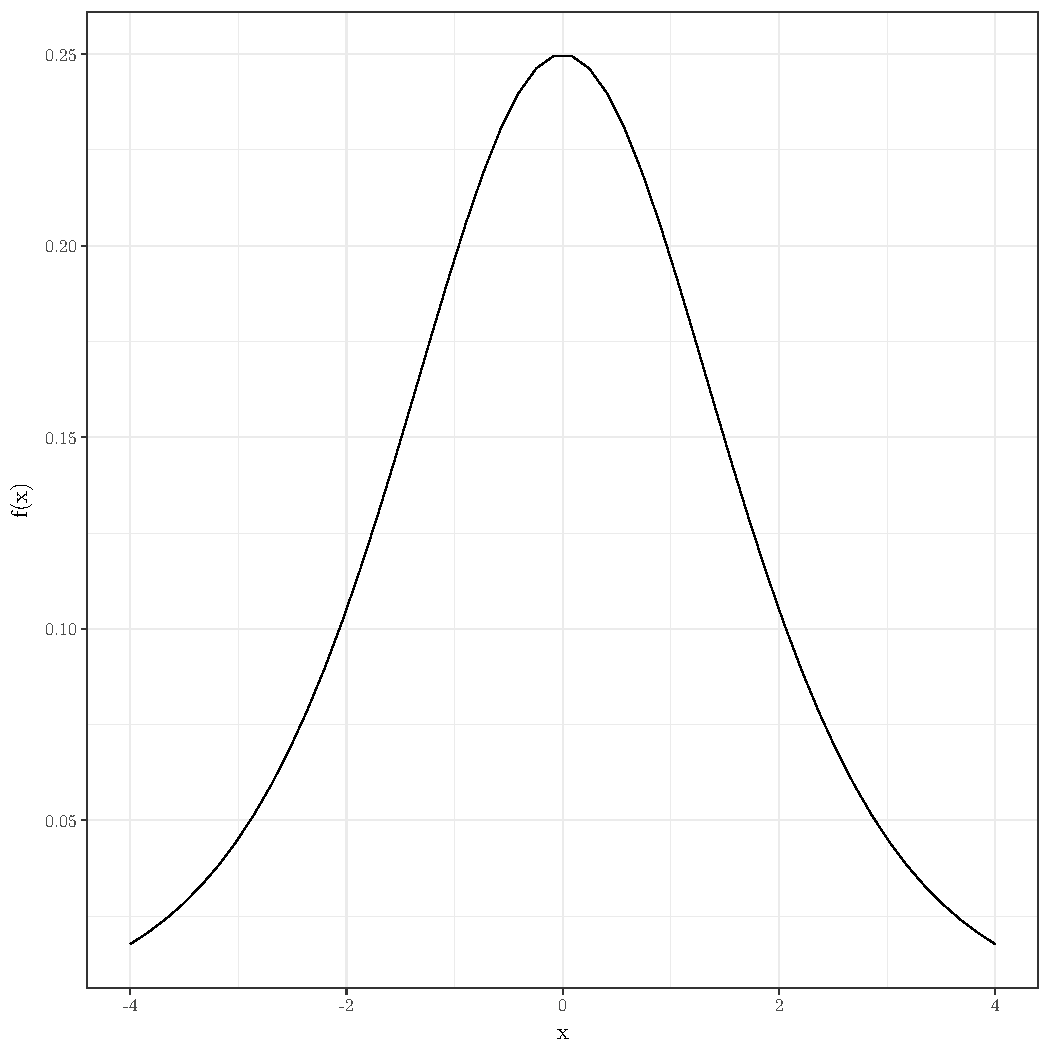
\includegraphics[scale=0.5]{auto_figures_tikz/2014_2015_fig_01_dlogis.pdf}
\end{center}
\end{minipage}


\end{enumerate}


\subsubsection*{Часть 2}

\begin{flushright}
 — Это невозможно! \\
— Нет. Это необходимо.\\
\textcopyright \hspace{0.1cm} Interstellar
\end{flushright}

\begin{enumerate}
\item
Алгоритм решения: рисуешь дерево $\rightarrow$ PROFIT

\begin{center}

 \begin{tikzpicture}[->,>=stealth',shorten >=1pt,auto,node distance=3cm,
  thick,main node/.style={circle,fill=blue!20,draw,font=\sffamily\Large\bfseries}]

  \node[main node] (1) {1};
  \node[main node] (2) [below of=1] {2};
  \node[main node] (3) [below of=2] {3};

  \path[every node/.style={font=\sffamily\small}]
    (1) edge [loop right] node {«не 6»} (1)
        edge [bend right] node[left] {«6»} (2)
    (2) edge [bend right] node[right] {«не 6»} (1)
        edge [above] node[left] {«6»} (3);
\end{tikzpicture}

\end{center}

Комментарии к построению дерева: состояние 1 — начальное, состояние 3 — конец игры, когда выпало две «шестерки» подряд. Заметим, что выпадение любой «нешестерки» в процессе игры приводит нас к состоянию, эквивалентному начальному.

Вероятность выпадения «шестерки» равна 1/6, «нешестерки» — 5/6.

Теперь мы готовы оседлать коня!

\begin{enumerate}
\item $\P(N = 1) = 0$ — невозможно за ход закончить игру.

$\P(N = 2) = \frac{1}{36}$

$\P(N = 3) = \frac{5}{6} \cdot \frac{1}{6} \cdot \frac{1}{6} = \frac{5}{216}$

\item А теперь будет видна вся сила рисования дерева:

Пусть $\E_1$ — число ходов, за которое мы ожидаем закончить игру, если игра начинается в состоянии 1, $\E_2$ — число ходов, за которое мы ожидаем закончить игру, если игра начинается в состоянии 2.

Получим два уравнения:
$\begin{cases} \E_2 = \frac{1}{6} \cdot 1 +  \frac{5}{6} (\E_1 + 1)   \\ \E_1 =  \frac{5}{6} (\E_1 + 1) + \frac{1}{6} ( \E_2 + 1) \end{cases} $

Решив эту систему, получим, что $\E_1 = 42$. А ведь это и есть $\E(N)$.

Аналогична логика для оставшихся мат. ожиданий.

Найдем математическое ожидание суммы набранных очков. Ясно, что если выпадает «не 6», то мы ждем 3 очка. Тогда переопределив $\E_1$ и $\E_2$ следующим образом: пусть $\E_1$ — число набранных очков, которое мы ожидаем получить за игру, если игра начинается в состоянии 1, $\E_2$ — число набранных очков, которое мы ожидаем получить за игру, если игра начинается в состоянии 2.

Новые два уравнения:
$\begin{cases} \E_2 = \frac{1}{6} \cdot 6 +  \frac{5}{6} (\E_1 + 3)   \\ \E_1 =  \frac{5}{6} (\E_1 + 3) + \frac{1}{6} ( \E_2 + 6) \end{cases} $

Решаем и получаем: $\E(S) = \E_1 = 147$

А можно было сделать еще круче! Выше показано, что  $\E(N) = 42$. А сколько мы ждем очков за 1 ход? 3.5! Тогда $\E(S) = \E(N) \cdot 3.5 = 147$

Применяя схожую логику для $\E(N^2)$:\\
\[\E(N^2) = \frac{5}{6} \cdot \E\left((N + 1)^2\right) + \frac{1}{6} \cdot \frac{5}{6}  \cdot \E\left((N + 2)^2\right) + \frac{1}{6} \cdot \frac{1}{6} \cdot 2^2\]

Учитывая, что $\E(N) = 42$, получим: $\E(N^2) = 3414$.

\item Veni, vidi, vici
\begin{center}
  \begin{tabular}{@{}cc@{}}
  \toprule
  $X_n$       & $6$ \\ \midrule
  $\P(\cdot)$ & $1$ \\ \bottomrule
  \end{tabular}
\end{center}

\end{enumerate}

\item
\begin{enumerate}
\item $\P(V = 1) = 1/30$, т.к. именно этому равна вероятность того, что Вовочка стоит ровно вторым в очереди;

$M = 1$ значит, что между Машенькой и Вовочкой ровно один человек в очереди. Если Вовочка находится от 3 (включительно) до 28 позиции в очереди, то для Машеньки есть две благоприятные позиции для события $M = 1$ (например, если Вовочка стоит на 15 месте, то благоприятные позиции для Машеньки — стоять либо 13-ой, либо 17-ой). Если же Вовочка стоит на других позициях в очереди, то для Машеньки существует ровно одна благоприятная позиция:

\[\P(M = 1) = \frac{26}{30} \cdot \frac{2}{29} +  \frac{4}{30} \cdot \frac{1}{29} = \frac{56}{30\cdot 29} = \frac{28}{435}\]

$M = V$ произойдет только, если Машенька стоит за Вовочкой. При этом для Машеньки существует только одна благоприятная позиция и только в том случае, что Вовочка стоит до 15 позиции (включительно):
\[\P(M = V) = \frac{1}{2} \cdot \frac{1}{29} = \frac{1}{58} \]

\item \[\E(V) = \frac{0 + 1 + \ldots + 29}{30} = \frac{30\cdot 14 + 15}{30} = 14.5\]

Для $\E(M)$ можно решить в лоб, и получится красивая сумма, а можно вот так:

Сначала случайно кинем Вовочку и Машеньку на две из 30 позиций в очереди. Образуется три отрезка: точки между Вовочкой и Машенькой и два крайних отрезка (может быть, отрезок из 0 точек). Затем будем закидывать в очередь на оставшиеся позиции случайно 28 оставшихся людей (назовем их «пропавшими»). Т.к. все броски были случайны (или из соображений симметрии, как хотите), вероятность попасть в отрезок между Машенькой и Вовочкой для «пропавшего» равна $1/3$, вне отрезка — соответственно $2/3$, и независима от остальных бросков (!).

Введем случайную величину $X_i$ для $i$-го «пропавшего», которая равна $1$, если он попал в отрезок между Машенькой и Вовочкой, $0$, если не попал:


\begin{center}
\begin{tabular}{ccc}
\toprule
$X_i$ & $1$ & $0$ \\ \midrule
$\P(\cdot)$ & $1/3$ & $2/3$ \\ \bottomrule
\end{tabular}

\end{center}


Легко считается: $\E(X_i) = 1/3$, $\E(X^2_i) = 1/3$, $\Var(X_i) = 1/3 - 1/9 = 2/9$.
Ясно, что $M = \sum_1^{28} X_i$. Тогда учитывая независимость $X_i$:

\[\E(M) = \frac{28}{3}\]
\[\Var(M) = \frac{56}{9}\]
\end{enumerate}

\item
Биномиальное распределение — \textit{À l’abordage!}.

Задача интерпретируется так: последний ход — это когда мы обратились к коробку, в котором нет спичек (то есть к одному коробку нужно обратиться $n+1$ раз).

\begin{enumerate}
\item Пусть $\xi$ — это случайная величина, обозначающая число оставшихся спичек в непустом коробке перед последним ходом.

Если $0<k \leqslant n$, будем считать успехом — попадание в коробок, к которому мы на последнем ходу игры (пустому коробку) обратились. До этого момента из него было вытащено $n$ спичек, а из другого $n-k$ спичек, то есть спички брались $2n - k$ раз.
Таким образом, перед последним ходом произошло $n$ успехов и $n-k$ неудач.
\[
\P(\xi = k) = C_{2n-k}^{n-k} = \left(\frac{1}{2}\right)^{n-k} \left(\frac{1}{2}\right)^{n} = C_{2n-k}^{n-k} \left(\frac{1}{2}\right)^{2n-k}
\]
Теперь нужно учесть, что на последнем ходе был выбран именно пустой коробок. Вероятность этого события — $1/2$, значит, искомая вероятность равна:
\[
\P(\text{в одном коробке осталось k спичек}) =  C_{2n-k}^{n-k} \left(\frac{1}{2}\right)^{2n-k} \cdot \frac{1}{2} = C_{2n-k}^{n-k} \left(\frac{1}{2}\right)^{2n-k+1}
\]
%Успехов — $n + 1$ (вытащено $n$ спичек, и на последнем ходу мы к нему обратились). По формуле Бернулли получаем следующее ($X$ — случайная величина, показывающая сколько спичек осталось в коробке, к которому мы не обратились на последнем ходу игры):
%\[\P(X = k) = C^{n+1}_{2n-k+1} \left(\frac{1}{2} \right)^{2n-k+1}\]

%Если $k = 0$, то мы вытащили все спички из обоих коробков к последнему ходу, и нам без разницы к какому коробку мы обратимся на последнем шагу, т.е.:
%\[\P(X = 0) =2 C^{n+1}_{2n+1} \left(\frac{1}{2} \right)^{2n+1}\]

\item Среднее спичек в другом коробке:

\[\E(X) = \sum \limits_{k=1}^{n} k \cdot C^{n-k}_{2n-k} \left(\frac{1}{2} \right)^{2n-k+1}\]


\end{enumerate}


\item
Для того чтобы количество упаковок, которые необходимо купить, равнялось 50, нужно чтобы ни одну из наклеек Покупатель не встретил дважды, поэтому:
\[
\P(X=50) = 1\cdot\frac{49}{50}\cdot\frac{48}{50}\cdot\dots\cdot\frac{1}{50} = \frac{49!}{50^{49}} \approx 3.4\cdot
10^{-21}\] \vspace{-1cm}

\hspace{10.5cm}\fcolorbox{ForestGreen}{white}{Dum spiro, spero!}\footnote[2]{Надежда умирает последней!}

Теперь введем понятие «шаг». Переход на новый шаг происходит в тот момент, когда покупатель получил наклейку, которой у него раньше не было. Начинаем с шага 0, когда нет ни одной наклейки, и шагать будем до 49, потому что в момент перехода на шаг 50 Покупатель получит последнюю необходимую наклейку и «прогулка» закончится. Введем случайную величину $X_q$ равную количеству покупок в течение шага номер $q$. Тогда $X = \sum \limits_{q=0}^{49}X_q$.  Найдем математическое ожидание $X_q$:
\[
\E(X_q) = \frac{n-q}{n}\cdot 1 + \frac{q}{n}\cdot\frac{n-q}{n}\cdot 2 + \left(\frac{q}{n}\right)^2\cdot\frac{n-q}{n}\cdot 3 + \ldots
\]
здесь $\frac{n-q}{n}$ —  это вероятность найти наклейку, которой еще нет, а $\frac{q}{n}$, соответственно — вероятность повториться. Вопрос теперь в том, как посчитать сумму:
\[
\E(X_q) = \frac{n-q}{n}\left( 1 + \frac{q}{n}\cdot 2 + \left(\frac{q}{n}\right)^2 \cdot 3 + \ldots\right) = \frac{n-q}{n}\cdot\sum\limits_{k=0}^{\infty}\left(\frac{q}{n}\right)^k(k+1)
\]

Можем выписать в столбик несколько первых членов вышестоящей суммы:
\[
\begin{array}{l}
\hspace{0.3cm}1 \\
\vspace{0.2cm}
\left(\frac{q}{n}\right)^1  + \left(\frac{q}{n}\right)^1  \\
\vspace{0.2cm}
\left(\frac{q}{n}\right)^2 + \left(\frac{q}{n}\right)^2  + \left(\frac{q}{n}\right)^2 \\
\left(\frac{q}{n}\right)^3 + \left(\frac{q}{n}\right)^3 + \left(\frac{q}{n}\right)^3 + \left(\frac{q}{n}\right)^3 \\
\hspace{0.1cm}\cdots\cdots\cdots\cdots\cdots\cdots\cdots\cdots\cdots\cdots\cdots
\end{array}
\]
Достаточно! Можем скомпоновать всю сумму другим способом, а именно — по столбцам. Заметим, что сумма элементов в каждом столбце это сумма бесконечно убывающей геометрической прогрессии с одним и тем же знаменателем $\frac{q}{n}$ и различными первыми членами. Соответственно:

\[
\sum\limits_{k=0}^{\infty}\left(\frac{q}{n}\right)^k(k+1) = \frac{1}{1-\frac{q}{n}} + \frac{\frac{q}{n}}{1-\frac{q}{n}} + \frac{\left(\frac{q}{n}\right)^2}{1-\frac{q}{n}} + \frac{\left(\frac{q}{n}\right)^3}{1-\frac{q}{n}} + \dots =
\]
\[
= \frac{1}{1-\frac{q}{n}}\left( 1 + \frac{q}{n} + \left(\frac{q}{n}\right)^2 + \left(\frac{q}{n}\right)^3 + \dots\right) = \frac{n}{n-q}\cdot\frac{n}{n-q} = \left( \frac{n}{n-q}\right)^2
\]

Таким образом, получаем, что:
\[
\E(X_q) = \frac{n-q}{n}\cdot \left( \frac{n}{n-q}\right)^2 = \frac{n}{n-q}
\]
\hspace{10cm} и это верно для любого q!

\[
\E(X) = \E\left(\sum \limits_{q=0}^{49}X_q\right) = \sum \limits_{q=0}^{49}\E(X_q) =
\frac{50}{50-0} + \frac{50}{50-1} + \dots + \frac{50}{50-49} = 50\left(\frac{1}{50} + \frac{1}{49} + \dots + 1\right) \approx
\]
\[
\approx 50\int\limits_{1}^{50}\frac{1}{x}\mathbf{d}x = 50\ln(50) \approx 195.5
\]

А теперь ещё одно решение:


Величины $X_q$ независимы (но по разному распределены). Если долго пришлось ждать $i$-го шага, это ничего не говорит о $j$-ом шаге. Величины $X_q$ имеют известный закон распределения — это число опытов до первого успеха при заданной вероятности успеха. Это геометрическое распределение, математическое ожидание которого равно $\frac{1}{p}$, а дисперсия: $\frac{1-p}{p^2}$, где $p$ — \vspace{0.2cm}  вероятность успеха.

А те, кто забыл, могут \textbf{проще решить} методом первого шага:
Если $X$ — число опытов до успеха при вероятности успеха $p$, то
\[
\E(X)=p\cdot 1 + (1-p)\cdot \E(X+1)
\]
Откуда $\E(X)=\frac{1}{p}$ и дело в шляпе :)
Аналогично:
\[
\E(X^2)=p\cdot 1^2 + (1-p) \cdot \E((X+1)^2)
\]
и решая, находим $\E(X^2)$.



\item
\begin{enumerate}
\item Необходимое и достаточное условие — старушка не должна занять чужое место. С вероятностью $\frac{1}{n}$ она угадает свое место, значит, для каждого входящего его место будет свободно и он туда сядет.\\
\textbf{Ответ:} $\frac{1}{n}$
\item Будем искать вероятность того, что последний человек не сядет на свое место.

Пусть $A_i = \{\text{Старушка села на  место } i\text{-го} \}$,  $B_{(i,j)} = \{i \text{-ый  пассажир сел на место } j\text{-ого} \}$

\[
P[n\text{-ый не сядет на свое место}] = \P(A_n) + P[A_{n-1}]P[B_{(n-1,n)}]+
\]
\[
+ P[A_{n-2}](P[B_{(n-2,n)}]
+ P[B_{(n-2,n-1)}]P[B_{(n-1,n)}]  ) + \dots
\]

Можем заметить, что:
\renewcommand{\labelitemi}{$\checkmark$}
\begin{itemize}
\item $\P[A_i] = P[A_j] = \frac{1}{n}$ $\forall \hspace{0.1cm} i, j$
\item $\P[B_{(n-1,n)}]=\frac{1}{2}$, потому что $n-1$-ый выбирает из двух оставшихся мест
\item $\P[B_{(n-2,n)}]
+ \P[B_{(n-2,n-1)}]P[B_{(n-1,n)}]  = \frac{1}{3} + \frac{1}{3}\cdot \frac{1}{2} = \frac{1}{2}$
\item
\begin{multline*}
\P[B_{(n-3,n)}] + \P[B_{(n-3,n-2)}](\P[B_{(n-2,n)}]+\P[B_{(n-2,n-1)}]\P[B_{(n-1,n)}])+\\
+ \P[B_{(n-3,n-1)}]\P[B_{(n-1,n)}] =   \frac{1}{4}+\frac{1}{4}\left(\frac{1}{3}+\frac{1}{3}\cdot\frac{1}{2}\right) +\frac{1}{4}\cdot \frac{1}{2} = \frac{1}{2}
\end{multline*}
\item И так далее до того момента, пока старушка не сядет на место первого человека, который заходит после нее, — всего $n-2$ вариантов.
\end{itemize}

Таким образом мы получаем сумму:
\[
\P[n\text{-ый не сядет на свое место}] = \frac{1}{n} + \frac{1}{n}\cdot \frac{1}{2} + \frac{1}{n}\cdot \frac{1}{2} + \dots = \frac{1}{n}  + \frac{1}{2n}(n-2) = \frac{1}{2}
\]
\begin{center}
\fcolorbox{ForestGreen}{white}{
Значит вероятность $\P[n\text{-ый сядет на свое место}] = 1 -\frac{1}{2} = \frac{1}{2}$}
\end{center}

А вот ещё один вариант решения:

\underline{Метод математической индукции:} допустим что это утверждение доказано для одного, двух и так далее до $k$ человек. Рассмотрим $k+1$ человека. Когда последний сядет на своё место? Если старушка сядет на своё место, а вероятность этого равна $\frac{1}{k+1}$ или, с вероятностью $\frac{1}{2}$ (по индукции), если старушка сядет на любое место кроме своего и последнего, то есть $\frac{1}{2}\cdot\frac{k-1}{k+1}$. В этом случае тот\vspace{0.2cm} пассажир, чье место  она заняла, становится старушкой, и мы получаем задачу при меньшем $k$. Складывая эти две дроби, получаем $\frac{1}{2} $.

Чтобы найти среднее число пассажиров, разобьем эту величину в сумму индикаторов: $Y_1$ — сел ли первый на место, $\dots$, $Y_n$ — сел ли $n$-ый на место (индикатор равен единице, если сел).

Стало быть $\E(Y)=\E(Y_1)+\E(Y_2)+\ldots+\E(Y_n)$. $\E(Y_n)=\frac{1}{2}$.

Почти аналогично можем рассуждать для предпоследнего:

База индукции: если пассажиров трое ($n=3$ включая старушку), то для предпоследнего вероятность сесть на своё место равна $\frac{2}{3}$.

Шаг индукции: допустим что для $3, 4, \ldots n$ пассажиров эта вероятность равна $\frac{2}{3}$.
Рассмотрим случай $(n+1)$-го пассажира.
Предпоследний сядет на своё место, если:

\renewcommand{\labelitemi}{\textbullet}

\begin{itemize}
\item старушка сядет на своё место или на место последнего $\frac{2}{n+1}$
\item в $\frac{2}{3}$ тех случаев, когда старушка сядет на место $2, 3, \ldots, (n-1)$, т.е. $\frac{2}{3}\cdot \frac{n-2}{n+1}$
складываем, получаем $\frac{2}{3}$.
То есть по индукции вероятность того, что предпоследний сядет на своё место равна $\frac{2}{3}$
\end{itemize}
И по аналогии можно увидеть, что вероятность того, что $k$-ый с конца пассажир сядет на своё место равна $k/(k+1)$

Если у нас $n$ пассажиров включая СС, то среднее количество севших на свои места (раскладывая с конца) равно \[\frac{1}{2}+\frac{2}{3}+\frac{3}{4}+\dots+\frac{n-1}{n}+\frac{1}{n}\]

\end{enumerate}

\end{enumerate}



\subsection{Контрольная работа 2. Базовый поток. 15.12.2014}


\begin{enumerate}
\item Ежемесячные расходы студенческой семьи Маши и Васи хорошо описываются случайным
вектором $(X,Y)$, ($X$ — расходы Маши, $Y$ — расходы Васи), имеющим равномерное
распределение в треугольнике, задаваемом ограничениями $\{0 \leq X, \; 0\leq Y, \; X+Y \leq 1 \}$.

Найдите:

\begin{enumerate}
\item Вероятность того, что совокупные расходы превысят половину бюджета, $\P(X+Y>1/2)$
\item Плотность распределения расходов Васи.
\item Вероятность того, что Машины расходы составили менее трети бюджета, если
известно, что Вася израсходовал более половины семейного бюджета.
\item Условную плотность распределения и условное математическое ожидание расходов Маши, при условии, что Вася израсходовал половину бюджета.
\item Математическое ожидание условного математического ожидания расходов Маши, $\E(\E(X|Y))$
\item Коэффициент корреляции расходов Маши и Васи
\end{enumerate}

\item Задана последовательность независимых случайных величин $X_1$, $X_2$, \ldots

\begin{tabular}{llll}
\toprule
$X_n$ & $-\sqrt{n}$ & $0$ & $\sqrt{n}$ \\ \midrule
$\P(\cdot)$ & $1/2n$ & $1-1/n$ & $1/2n$ \\
\bottomrule
\end{tabular}

\begin{enumerate}
\item Сформулируйте закон больших чисел. Выполняется ли для данной последовательности
закон больших чисел?
\item Запишите неравенство Чебышёва. Оцените вероятность того, что модуль среднего
значения по $n$ наблюдениям не превысит $1$, $\P(|\bar X_n| \leq 1)$
\item Сколько членов последовательности необходимо взять, чтобы вероятность того, что
модуль среднего значения не превысит $1$, была не менее $0.9$, $\P(|\bar X_n| \leq 1)\geq 0.9$
\end{enumerate}

\item Размер выплат каждому клиенту банка — случайная величина с математическим
ожиданием, равным 5000 ед. и среднеквадратическим отклонением, равным 2000 ед.
Выплаты отдельным клиентам независимы. Сколько должно быть наличных денег в банке,
чтобы с вероятностью 0.95 денег хватило на обслуживание 60 клиентов?

\item Рекламная компания хочет оценить вероятность $p$, с которой адресная реклама приводит к
заявке. С этой целью она  рассылает $n$ рекламных проспектов. Обозначим за $\hat p$ отношение
числа поданных заявок к числу разосланных проспектов $n$. С помощью теоремы Муавра–Лапласа и неравенства Чебышёва определите:
\begin{enumerate}
\item  Сколько нужно разослать рекламных проспектов, для того чтобы $\hat p$ отличалось от
истинной вероятности $p$ не более, чем на $0.1$ с вероятностью не меньшей $0.99$
\item С какой точностью $\varepsilon$ удастся оценить $p$ с вероятностью 0.99, если разослана 1000
проспектов, т.е. $\P(|\hat p - p|\leq \varepsilon)\geq 0.99$?
\end{enumerate}
\end{enumerate}





\subsection{Контрольная работа 2. Базовый поток. 15.12.2014, решение}


\begin{enumerate}
\item
\begin{enumerate}
\item
Так как $(X, Y)$ имеют совместное равномерное распределение, $\P\left\{X+Y > \frac{1}{2}\right\}$ можно рассчитать как отношение соответствующих площадей:
\begin{center}
\definecolor{zzttqq}{rgb}{0.6,0.2,0.}
\begin{tikzpicture}[line cap=round,line join=round,>=triangle 45,x=5.692307692307692cm,y=5.692307692307692cm]
\draw[->,color=black] (-0.1,0.) -- (1.2,0.);
\foreach \x in {,0.2,0.3,0.4,0.5,0.6,0.7,0.8,0.9,1.,1.1}
\draw[shift={(\x,0)},color=black] (0pt,2pt) -- (0pt,-2pt) node[below] {\footnotesize $\x$};
\draw[->,color=black] (0.,-0.1) -- (0.,1.2);
\foreach \y in {0.2,0.3,0.4,0.5,0.6,0.7,0.8,0.9,1.,1.1}
\draw[shift={(0,\y)},color=black] (2pt,0pt) -- (-2pt,0pt) node[left] {\footnotesize $\y$};
\draw[color=black] (0pt,-10pt) node[right] {\footnotesize $0$};
\clip(-0.1,-0.1) rectangle (1.2,1.2);
\fill[color=zzttqq,fill=zzttqq,fill opacity=0.1] (0.,0.5) -- (0.5,0.) -- (1.,0.) -- (0.,1.) -- cycle;
\draw (0.,1.)-- (1.,0.);
\draw [color=zzttqq] (0.,0.5)-- (0.5,0.);
\draw [color=zzttqq] (0.5,0.)-- (1.,0.);
\draw [color=zzttqq] (1.,0.)-- (0.,1.);
\draw [color=zzttqq] (0.,1.)-- (0.,0.5);
\draw (0.344196516991,0.436512272899) node[anchor=north west] {$S_0$};
\draw (0.129676687465,0.218325437741) node[anchor=north west] {$S_1$};
\draw (0.0233335241101,1.16441289103) node[anchor=north west] {$y$};
\draw (1.06109611823,0.08) node[anchor=north west] {$x$};
\end{tikzpicture}
\end{center}

Соответственно: \[\P\left(X+Y > \frac{1}{2}\right) = \frac{S_0}{S_0+S_1} = \frac{0.5-S_1}{0.5} = \frac{\frac{1}{2}-\frac{1}{8}}{\frac{1}{2}} = \frac{3}{4}\]

\item
\[
f_Y(y) = \int \limits_{0}^{1-y} f_{XY}(x,y) dx
\]

Поэтому, нам сначала нужно найти $f_{XY}(x,y)$, которая для равномерного распределения должна быть константой. Это можно сделать из условия:
\[
\int\limits_{0}^{1}\int \limits_{0}^{1-x} f_{XY}(x, y) dxdy = \int\limits_{0}^{1}\int \limits_{0}^{1-x} C dxdy = 1 \Rightarrow
\]
\[
\int\limits_{0}^{1}\int \limits_{0}^{1-x} C dxdy = \int\limits_{0}^{1} C(1-x) dx = \left. \left( Cx-C\frac{x^2}{2}\right) \right| _{0}^{1} =
 \frac{C}{2}  = 1\]

 Откуда имеем $f_{XY}(x, y) = C = 2$. Теперь можем найти плотность распределения расходов Васи:
 \[ f_Y(y) = \int \limits_{0}^{1-y} 2 dx = 2(1-y) \]



\item В данном случае площади немного другие, но смысл тот же:

\begin{center}
\definecolor{zzttqq}{rgb}{0.6,0.2,0.}
\begin{tikzpicture}[line cap=round,line join=round,>=triangle 45,x=5.692307692307692cm,y=5.692307692307692cm]
\draw[->,color=black] (-0.1,0.) -- (1.2,0.);
\foreach \x in {,0.2,0.3,0.4,0.5,0.6,0.7,0.8,0.9,1.,1.1}
\draw[shift={(\x,0)},color=black] (0pt,2pt) -- (0pt,-2pt) node[below] {\footnotesize $\x$};
\draw[->,color=black] (0.,-0.1) -- (0.,1.2);
\foreach \y in {,0.2,0.3,0.4,0.5,0.6,0.7,0.8,0.9,1.,1.1}
\draw[shift={(0,\y)},color=black] (2pt,0pt) -- (-2pt,0pt) node[left] {\footnotesize $\y$};
\draw[color=black] (0pt,-10pt) node[right] {\footnotesize $0$};
\clip(-0.1,-0.1) rectangle (1.2,1.2);
\fill[color=zzttqq,fill=zzttqq,fill opacity=0.1] (0.,0.5) -- (0.,1.) -- (0.333333333333,0.666666666667) -- (0.333333333333,0.5) -- cycle;
\draw (0.,1.)-- (1.,0.);
\draw[dashed] (1/3, 2/3) -- (1/3,0);
\draw (0.1004007648034,0.729040237615) node[anchor=north west] {$S_0$};
\draw (0.343364031073,0.5908861537646) node[anchor=north west] {$S_1$};
\draw (0.0233335241101,1.16441289103) node[anchor=north west] {$y$};
\draw (1.06109611823,0.08) node[anchor=north west] {$x$};
\draw (0.,0.5)-- (0.5,0.5);
\draw [color=zzttqq] (0.,0.5)-- (0.,1.);
\draw [color=zzttqq] (0.,1.)-- (0.333333333333,0.666666666667);
\draw [color=zzttqq] (0.333333333333,0.666666666667)-- (0.333333333333,0.5);
\draw [color=zzttqq] (0.333333333333,0.5)-- (0.,0.5);
\end{tikzpicture}
\end{center}


\[\P\left( \left. X<\frac{1}{3} \hspace{1mm} \right| Y>\frac{1}{2}\right) = \frac{S_0}{S_0+S_1} = \frac{\frac{1}{8} - S_1}{\frac{1}{8}} = \frac{\frac{1}{8}-\frac{1}{72}}{\frac{1}{8}} = \frac{8}{9}\]

\item При $Y = \frac{1}{2}$, $X$ распределен равномерно от 0 до $\frac{1}{2}$, поэтому его плотность равна \[f_X(x) = \frac{1}{\frac{1}{2} - 0} = 2\]
Соответственно, условное математическое ожидание:
\[
\E \left( X| Y =\frac{1}{2}\right) = \frac{1}{4}
\]

\item $\E(\E(X|Y)) = \E(X)$, а маргинальную функцию плотности для $X$ мы можем найти так же, как искали для $Y$, и получим $f_X(x) = 2(1-x)$. Отсюда:
\[
\E(X) = \int \limits_{0}^{1} 2x(1-x)dx = \left .\left(x^2 - \frac{2}{3}x^3\right) \right|^{1}_{0} = \frac{1}{3}
\]

\item Если вспомнить формулу для корреляции:
\[
\rho_{XY} = \frac{\Cov(X, Y)}{\sigma_X\sigma_Y}  = \frac{\E(XY) - \E(X)\E(Y)}{\sigma_X\sigma_Y}
\]

то станет более-менее очевидно, что надо найти $\E(XY)$ и дисперсии $X$ и $Y$.

\[
\E(XY) = \int \limits_{0}^{1} \int \limits_{0}^{1-x} 2xy dxdy = \int \limits_{0}^{1} 2xdx \int \limits_{0}^{1-x}ydy =  \int \limits_{0}^{1}x(x^2-2x+1)dx =
\]
\[
= \left. \left(\frac{x^4}{4} - \frac{2}{3}x^3 + \frac{x^2}{2}\right) \right|^{1}_{0} = \frac{3}{4}-\frac{2}{3} = \frac{1}{12}
\]

Соответственно:

\[
\Cov(X, Y) = \frac{1}{12} - \frac{1}{3}\cdot \frac{1}{3} = -\frac{1}{36}
\]

Найдем теперь дисперсии $X$ и $Y$ (они будут одинаковыми, как и математические ождания, в силу симметрии):

\[
\E(X^2) = \int \limits_{0}^{1} 2x^2(1-x)dx = \left. \left( \frac{2}{3}x^2 - \frac{x_4}{2} \right) \right|_{0}^{1} = \frac{1}{6}
\]

Поэтому:
\[
\Var[X] = \E(X^2) - (\E(X))^2 = \frac{1}{6} - \frac{1}{9} = \frac{1}{18}
\]

Теперь наконец-то можем найти корреляцию:
\[
\rho_{XY} = -\frac{\frac{1}{36}}{\sqrt{\frac{1}{18}}\sqrt{\frac{1}{18}}} = -\frac{1}{2}
\]
\end{enumerate}

\item

\begin{enumerate}

\item Закон больших чисел гласит, что $\bar{X} \rightarrow
\E(X)$ при $n\rightarrow \infty$. Проверим его выполнение в данном случае:
\[
\E(X_n) = \frac{1}{2n}(-\sqrt{n}) + \left(1-\frac{1}{n}\right)\cdot0 + \frac{1}{2n}\sqrt{n} = 0
\]

\[
\lim\limits_{n\rightarrow\infty} \bar{X} = \lim\limits_{n\rightarrow\infty} \frac{X_1 +\dots + X_n}{n} = 0
\]
так как числитель ограничен, а знаменатель бесконечно возрастает.
Видим, что ЗБЧ в данном случае, конечно, выполняется.

Как вариант, можно было сказать, что дисперсия ограничена, и из этого также следует выполнение ЗБЧ.
\item Неравенство Чебышева:
\[
\P(|X-\E(X)|\geqslant \varepsilon) \leqslant \frac{\Var(X)}{\varepsilon^2}
\]

Соответственно, искомую вероятность можем оценить следующим образом:
\[
\P(|\bar{X}| \leqslant 1) = 1 -\P(|\bar{X}| \geqslant 1) \Rightarrow \P(|\bar{X}| \leqslant 1) \geqslant 1 - \frac{\Var[\bar{X}]}{1}
\]
\[
\Var[\bar{X}] = \Var\left(\frac{\sum\limits_{i=1}^{n} X_i}{n}\right) = \frac{1}{n^2}\sum \limits_{i=1}^{n} \Var{X_i}
\]
В свою очередь:

\[
\E(X_i^2) = 2\cdot\frac{1}{2n}\cdot n + \left(1-\frac{1}{n}\right)\cdot0 = 1 \Rightarrow \Var[X_i] = 1 \Rightarrow \Var[\bar{X}] = \frac{1}{n}
\]

Поэтому:
\[
\P(|\bar{X}| \leqslant 1)\geqslant 1 - \frac{1}{n}
\]

\item  \[1 - \frac{1}{n} = 0.9  \Rightarrow n = 10\]

\end{enumerate}

\item

Обозначим за $R$ — необходимое количество наличных денег в банке. Пусть $X$ — случайная величина, показывающее размер суммарной выплаты $60$ ($n$ — достаточное большое для применения ЦПТ) клиентам. Ясно, что т.к. выплаты отдельным клиентам независимы: \( \E X = 60 \cdot 5000 = 3\cdot 10^5 \); \( \Var X = 60 \cdot 2000^2 = 2.4 \cdot 10^8 \); \( \sigma_X = \sqrt{2.4} \cdot 10^4 \approx 1.55 \cdot 10^4\)

Теперь по ЦПТ:
\[\P(R \geqslant X) = 0.95 \]
\[\P \left(\frac{X - \E X}{\sigma_X} \leqslant \frac{R - \E X}{\sigma_X} \right) = 0.95 \]
\[ \P \left( Z \leqslant \frac{R - 3 \cdot 10^5}{1.55 \cdot 10^4} \right) = 0.95 \]
Слева функция распределения; подставляя 95-\% квантиль стандартного нормального распределения, получаем:
\[ \frac{R - 3 \cdot 10^5}{1.55 \cdot 10^4} = 1.64 \]
\[ R = 325420 \]


\item

\begin{enumerate}
\item По предельной теореме Муавра-Лапласа:
\[ \frac{\hat{p} - p}{\sqrt{p(1-p)/n}} \sim N (0,1) \]
\[ \P \left( \frac{|\hat{p} - p|}{\sqrt{p(1-p)/n}} \leqslant \frac{0.1}{\sqrt{p(1-p)/n}} \right) \geqslant 0.99 \]
\[ \P \left( |Z| \leqslant \frac{0.1}{\sqrt{p(1-p)/n}} \right) \geqslant 0.99 \]
Из симметричности стандартного нормального распределения и зная его 99.5-\% квантиль, равный приблизительно 2.58, получаем:
\[ \frac{0.1}{\sqrt{p(1-p)/n}} \geqslant 2.58 \]
\[ \frac{\sqrt{n}}{\sqrt{p(1-p)}} \geqslant \frac{2.58}{0.1} \]
\[ \sqrt{n} \geqslant \frac{2.58}{0.1} \sqrt{p(1-p)} \]
\[ n \geqslant 665.64 \cdot p(1-p) \]

С помощью неравенства Чебышева:
\[ \P \left( |\hat{p} - p| \leqslant 0.1 \right) \geqslant 0.99 \]
\[ \P \left( |\hat{p} - p| \geqslant 0.1 \right) \leqslant 0.01 \]
Теперь просто смотрим на неравенство Чебышева и на строчку выше, на неравенство Чебышева и на строчку выше\ldots
\[ \frac{p(1-p)/n}{0.1^2} = 0.01\]
\[ n = 10^4 p(1-p) \]
Принимаются оба ответа!

\item По предельной теореме Муавра-Лапласа:
\[ \P \left( \frac{|\hat{p} - p|}{\sqrt{p(1-p)/n}} \leqslant \frac{\varepsilon}{\sqrt{p(1-p)/1000}} \right) \geqslant 0.99 \]
\[ \P \left( |Z| \leqslant \frac{\varepsilon}{\sqrt{p(1-p)/1000}} \right) \geqslant 0.99 \]
Аналогично пункту 1:
\[ \frac{\varepsilon}{\sqrt{p(1-p)/1000}} \geqslant 2.58 \]
\[ \varepsilon \geqslant 0.082 \sqrt{p(1-p)} \]

С помощью неравенства Чебышева:
\[ \P \left( |\hat{p} - p| \leqslant \varepsilon \right) \geqslant 0.99 \]
\[ \P \left( |\hat{p} - p| \geqslant \varepsilon \right) \leqslant 0.01 \]
Аналогично пункту 1:
\[ \frac{p(1-p)/1000}{\varepsilon^2} = 0.01\]
\[ \varepsilon^2 = \frac{p(1-p)}{10} \]
\[ \varepsilon = \sqrt{\frac{p(1-p)}{10}} \approx 0.316 \sqrt{p(1-p)} \]

\end{enumerate}

Нужно было показать, как мастерство владения теоремой Муавра-Лапласа, так и неравенством Чебышева.


\end{enumerate}


\subsection{Праздник номер 2, i-поток, 15.12.2014}

Time: 180 min

\begin{enumerate}
\item Вася может получить за экзамен равновероятно либо $8$ баллов, либо $7$ баллов. Петя может получить за экзамен либо $8$ баллов — с вероятностью $1/3$; либо $7$ баллов — с вероятностью $2/3$. Известно, что корреляция их результатов равна $0.7$.

Какова вероятность того, что Петя и Вася покажут одинаковый результат?

\item В  городе Туме проводят демографическое исследование семейных пар. Стандартное отклонение возраста мужа оказалось равным 5 годам, а стандартное отклонение возраста жены — 4 годам. Найдите корреляцию возраста жены и возраста мужа, если стандартное отклонение разности возрастов оказалось равным 2 годам. В каких пределах лежит вероятность того, что возраст случайно выбираемого женатого мужчины отклоняется от своего математического ожидания больше чем на 10 лет?


\item На окружности единичной длины случайным образом равномерно и независимо друг от друга выбирают две дуги: длины $0.3$ и длины $0.4$.
\begin{enumerate}
\item  Найдите функцию распределения длины пересечения этих отрезков
\item Найдите среднюю длину пересечения
\end{enumerate}


\item  Совместная функция плотности величин $X$ и $Y$ имеет вид
\begin{equation}
\nonumber
f(x,y)=\begin{cases}
2(x^3+y^3), \text{ если } x\in [0;1], y\in [0;1] \\
0, \mbox{ иначе}
\end{cases}
\end{equation}
\begin{enumerate}
\item Найдите $\P(X+Y>1)$
\item Найдите $\Cov(X,Y)$
\item Являются ли величины $X$ и $Y$ независимыми?
\item Являются ли величины $X$ и $Y$ одинаково распределенными?
\end{enumerate}



\item Изначально цена акций компании «Пумперникель» равна $X_0=1000$ рублей. Каждый последующий день в течение 100 дней цена равновероятно может вырасти на 2 рубля или упасть на 1 рубль. Обозначим цену акции через $n$ дней как $X_n$.
\begin{enumerate}
\item Чему равны математическое ожидание и дисперсия изменения цены за отдельный день?
\item Найдите $\E(X_n)$, $\Var(X_n)$, $\Cov(X_n, X_k)$
\item Сформулируйте центральную предельную теорему
\item Примерно найдите вероятность $\P(X_{100}>1060)$
\item Биржевой игрок Вениамин утверждает, что через 100 дней с вероятностью 95\% цена акций «Пумперникель» не опустится ниже $a$. Чему равно $a$?
\end{enumerate}
\item  Сэр Фрэнсис Гальтон —  учёный XIX-XX веков, один из основоположников как
генетики, так и статистики — изучал, среди всего прочего, связь между ростом детей и родителей.  Он исследовал данные о росте 928 индивидов. Обозначим $X_1$ — рост случайного человека, а $X_2$ — среднее арифметическое роста его отца и матери. По результатам исследования Гальтона:


\[
\begin{pmatrix}
X_1 \\
X_2
\end{pmatrix}
\sim
\cN\left[
\begin{pmatrix}
68.1 \\
68.3
\end{pmatrix};
\begin{pmatrix}
6.3 & 2.1 \\
2.1 & 3.2
\end{pmatrix}
\right]
\]

\begin{enumerate}
\item Обратите внимание на то, что дисперсия роста детей выше дисперсии среднего роста
родителей. С чем это
может быть связано? Учтите, что рост детей измерялся уже по достижении
зрелости, так что разброс не должен быть связан с возрастными различиями.
\item Рассчитайте корреляцию между $X_1$ и $X_2$
\item Один дюйм примерно равен $2.54$ сантиметра. Пусть $X_1'$ и $X_2'$ — это те же $X_1$ и $X_2$, только измеренные в сантиметрах. Найдите вектор математических ожиданий и ковариационную матрицу вектора $X'=(X_1', X_2')$.
\item Определите, каков ожидаемый рост и дисперсия роста человека, средний рост родителей которого составляет 72 дюйма?
\item Найдите вероятность того, что рост человека превысит 68 дюймов, если средний рост его родителей равен 72 дюймам. Подсказка: используйте предыдущий пункт и нормальность распределения!
\end{enumerate}

%\item Пуассоновское казино. В пуассоновском казино сигнальная лампочка загорается согласно пуассоновскому потоку в среднем один раз в минуту. В любой момент азартный игрок Вениамин может нажать кнопку. Нажать кнопку Вениамин может только один раз. Вениамин срывает джек-пот,

\item Звонки поступают в пожарную часть согласно пуассоновскому потоку в среднем $2$~раза в час. Предположим, что после получения звонка пожарная часть занята тушением пожара случайное время равномерно распределённое от получаса до часа. В это время звонки перенаправляются в соседнюю пожарную часть.

Пожарная часть только-только начала работать и готова принимать звонки.
\begin{enumerate}
\item Какова вероятность того, что за ближайший час не поступит звонков?
\item Какова вероятность того, что за ближайший час не будет перенаправленных звонков?
\item Найдите закон распределения количества звонков до первого перенаправленного звонка.
\end{enumerate}

\item  Судьба Дон-Жуана


У Дон-Жуана $n$  знакомых девушек, и их всех зовут по-разному. Он пишет
им $n$  писем, но по рассеянности раскладывает их в конверты
наугад. Случайная величина $X$ обозначает количество девушек, получивших письма, адресованные лично им.

\begin{enumerate}
\item Найдите $\E(X)$, $\Var(X)$
\item Какова при большом $n$ вероятность того, что хотя бы одна девушка получит письмо, адресованное ей?
\end{enumerate}

\item Игла Бюффона

Плоскость разлинована параллельными линиями через каждый сантиметр. Случайным образом на эту плоскость бросается иголка длины $a<1$.

\begin{enumerate}
\item Какова вероятность того, что иголка пересечёт какую-нибудь линию?
\item Предложите вероятностный способ оценки числа $\pi$
\end{enumerate}


\end{enumerate}


\subsection{Решение. Праздник номер 2, i-поток}

\begin{enumerate}
\item
Пусть $X$ — оценка Пети, $Y$ — оценка Васи. Тогда исходя из условия:
\begin{center}

\begin{tabular}{ccc}
\toprule
$X$ & $7$ & $8$ \\ \midrule
$\P(\cdot)$ & $\frac{1}{2}$ & $\frac{1}{2}$ \\ \bottomrule
\end{tabular}
\hspace{1cm}
\begin{tabular}{ccc}
\toprule
$Y$ & $7$ & $8$ \\ \midrule
$\P(\cdot)$ & $\frac{2}{3}$ & $\frac{1}{3}$  \\ \bottomrule
\end{tabular}
\end{center}

Теперь можем найти математические ожидания и дисперсии:
\[
\E(X) = \frac{15}{2}, \hspace{0.5cm} \E(Y) = \frac{22}{3} \Rightarrow
\]
\[
\Var[X] = \frac{1}{2}\cdot 64 + \frac{1}{2}\cdot 49 - \left(\frac{15}{2}\right)^2 = \frac{1}{4}
\]
\[
\Var[Y] = \frac{1}{3}\cdot 64 + \frac{2}{3}\cdot 49 - \left(\frac{22}{3}\right)^2 = \frac{2}{9}
\]

Теперь из формулы для корреляции мы можем найти $\E(XY)$:

\[
0.7 = \frac{\E(XY)-\frac{15}{2}\cdot\frac{22}{3}}{\sqrt{\frac{1}{4}}\sqrt{\frac{2}{9}}} \Rightarrow \E(XY) \approx 55.16499
\]

Можем составить табличку для совместного распределения, немножко подумав:

\begin{center}
\begin{tabular}{@{}lccr@{}}
\toprule
$Y$ \textbackslash $X$ & $7$             & $8$             & $\sum$        \\ \midrule
$7$                              & $p$             & $\frac{1}{2}-p$ & $\frac{1}{2}$ \\
$8$                              & $\frac{2}{3}-p$ & $p-\frac{1}{6}$ & $\frac{1}{2}$ \\
$\sum$                           & $\frac{2}{3}$   & $\frac{1}{3}$   &               \\ \bottomrule
\end{tabular}
\end{center}

\[
\E(XY) = 49p+56\left(\frac{1}{2} - p + \frac{2}{3}-p\right) + 64\left(p-\frac{1}{6}\right) = 55.16499
\]

\[
\Rightarrow p \approx 0.4983233 \Rightarrow \P(X=Y) = p + p-\frac{1}{6} = 0.8299799
\]



\item

Пусть $M$ — возраст мужа, $F$ — возраст жены. Тогда из условия:
\[
\Var(M-F) = \Var(M) + \Var(F) - 2\Cov(M, F) = 4 \Rightarrow \Cov(M, F) = \frac{37}{2}
\]

\[
\rho_{MF} = \frac{\frac{37}{2}}{5\cdot4} = \frac{37}{40}
\]


Согласно неравенству Чебышева:
\[
\P(|M-\E(M)|\geqslant10) \leqslant\frac{\Var(M)}{10^2} = 0.25
\]

Поэтому данная вероятность лежит в пределах $(0, 25]$.

\renewcommand{\labelenumii}{(\alph{enumii})}
\item
\begin{enumerate}
\item Пусть $X$ — длина пересечения. Требуется найти $\P(X\leqslant x)$. Рассмотрим расположение центров отрезков относительно друг друга:

\begin{center}
\definecolor{zzttqq}{rgb}{0.6,0.2,0.}
\begin{tikzpicture}[line cap=round,line join=round,>=triangle 45,x=7cm,y=7]
\draw[color=black] (0.,0.) -- (1.1,0.);
\foreach \x in {0,0.5,0.3,1.1}
\draw[shift={(\x,0)},color=black, line width= 1pt] (0pt,2pt) -- (0pt,-2pt) node[below] {};
\draw (0.25,0.) node[circle, inner sep = 1pt,  fill] {};
\draw (0.7,0.) node[circle, inner sep = 1pt,  fill] {};
\draw[<->, color = black] (0,-2) -- (0.25, -2) ;
\draw[<->, color = black] (0.25,-2) -- (0.7, -2) ;
\draw[<->, color = black] (0.7,-2) -- (1.1, -2) ;
\draw[color=black, dashed] (0,0) -- (0,-2);
\draw[color=black, dashed] (0.25,0) -- (0.25,-2);
\draw[color=black, dashed] (0.7,0) -- (0.7,-2);
\draw[color=black, dashed] (1.1,0) -- (1.1,-2);
\draw (0.125,-2) node[below] {0.15};
\draw (0.4,-2) node[below] {$R$};
\draw (0.8,-2) node[below] {0.2};
\draw[color = red, line width = 2pt] (0.3, 0) -- (0.5, 0);

\end{tikzpicture}
\end{center}

Заматим, что $X = 0.15-(R-0.2) = 0.35-R$. Однако, $R \sim U\left[0, \frac{1}{2}\right]$. Можно представить, что эти точки бросают на окружность по очереди, тогда расстояние между ними не может превышать $\frac{1}{2}$ и распределено равномерно. Имеем:
\[
\P(X \leqslant x) = \P(0.35-R\leqslant x) = \P(R \geqslant 0.35-x) = \frac{0.5-0.35+x}{0.5} = 0.3+2x
\]

Строго говоря, длина пересечения не может быть больше 0.3 по понятным причинам, поэтому функция распределения выглядит так:
\[
F(x) = \begin{cases}
0.3+2x, & x < 0.3\\
1, & x \geqslant 0.3
\end{cases}
\]

\item Зная функцию распределения, можем найти плотность:
\[f_X(x) = \begin{cases}
2, & x < 3\\
0, & \text{else}
\end{cases}\]

Сответственно:
\[
\E(X) = \int \limits_{0}^{0.3} 2x dx = \left.  x^2 \right|_{0}^{0.3} = 0.09
\]
\end{enumerate}



\item

\begin{enumerate}
\item \[\P(X+Y > 1) = \iint \limits_{\mathcal{G}}2(x^3+y^3)dxdy = \int \limits_{0}^{1} dx \int \limits_{1-x}^{1}2(x^3+y^3)dy = \ldots  = 0.8\]
\item Для того, чтобы найти ковариацию, придется найти :
\[\E(X) = \int\limits_{0}^{1} dx \int\limits _{0}^{1}2x(x^3+y^3)dy = \ldots = 0.65\]
\[\E(Y) = \int\limits_{0}^{1} dy \int\limits_{0}^{1}2y(x^3+y^3)dx = \ldots = 0.65 \]
\[\E(XY) = \int\limits_{0}^{1}dx\int\limits_{0}^{1}2xy(x^3+y^3)dy = \ldots = 0.4\]

Ну а потом все просто: $\Cov(X, Y) = \E(XY) - \E(X)\E(Y) = -0.0225$

\item Проверить свойство функций плотности $f_XY(x, y) = f_X(x)\cdot f_Y(y)$, а если $\Cov(X, Y) \ne 0$, то сразу зависимы. Здесь — зависимы.
\item Да, являются.
\end{enumerate}


\item
Для этой задачи аккуратно нужно писать \( \left(\Delta X \right)_j \), но так как приращения цен независимы (см. биномиальная модель рынка в интернетах) будем писать \( \Delta X \).
\begin{enumerate}
\item \[\E (\Delta X) = 2 \cdot \frac{1}{2} - 1 \cdot \frac{1}{2} = \frac{1}{2} \]
\[\E (\Delta X)^2 = 4 \cdot \frac{1}{2} + 1 \cdot \frac{1}{2} = \frac{5}{2} \]
\[\Var (\Delta X) = \frac{5}{2} - \left(\frac{1}{2}\right)^2 = \frac{10-1}{4}=\frac{9}{4} \]
\item \[\E (X_n) = \E \left(1000 + n\Delta X \right)  = 1000 + n \E \Delta X = 1000 + 0.5 n     \]
\[ \Var (X_n) = n \Var (\Delta X) = n \frac{9}{4}  \]
\[ \Cov (X_n, X_k) = \Cov \left(X_k, X_k + (n-k) \Delta X \right)     \]
Так как цена в момент $k$ никак не связана с последующими случайными блужданиями, то:
\[ \Cov (X_n, X_k) = \Cov \left(X_k, X_k + (n-k) \Delta X \right) =  \Cov \left(X_k, X_k \right) + 0 = \Var X_k = k \frac{9}{4}    \]
\item Заметим, что для самих цен акций ЦПТ мы формулировать не можем ввиду того, что случайные величины коррелированы, не i.i.d. Зато мы можем сформулировать ее для независимых приращений!

\( \left(\Delta X \right)_1, \ldots, \left(\Delta X \right)_{k} \) — последовательность i.i.d. случайных величин (при большом $k$) с конечными математическим ожиданием \(1/2 \) и стандартным отклонением \(3/2 \). Пусть также \( S_k = \sum_{i=1}^k \left(\Delta X \right)_j \). Тогда формулировка ЦПТ:
\[ \frac{S_k - k/2}{3/2 \sqrt{k}} \sim \cN(0,1)    \]
\item Воспользуемся результатом ЦПТ!
\[\P(X_{100} > 1060) = \P (1000 + S_{100} > 1060) = \P(S_{100} >60) = \]
\[ = \P \left(\frac{S_{100} -50 }{3/2\cdot 10} > \frac{60-50}{3/2 \cdot 10}\right) = \P \left(Z > \frac{2}{3}\right) = 1-pnorm(2/3) \approx 0.25   \]

\item \[ \P \left(1000 + S_{100} > a \right) = 0.95              \]
\[ \P \left( S_{100} < a-1000 \right) = 0.05              \]
Используя ЦПТ:
\[ a-1000 = qnorm(0.05, mean = 50, sd = 15 )            \]
\[ a \approx 1025.33   \]
\end{enumerate}

\item
\[\begin{pmatrix}
X_1 \\
X_2
\end{pmatrix} \sim \cN \left( \begin{pmatrix}
68.1 \\
68.3
\end{pmatrix} ; \begin{pmatrix}
6.3 & 2.1 \\
2.1 & 3.2
\end{pmatrix}                   \right)\]

\begin{enumerate}
\item \href{http://johnhawks.net/explainer/stats/heritability-and-stature/}{Смотреть здесь}
\item \[ \Corr(X_1, X_2) = \frac{\Cov(X_1, X_2)}{\sigma_{X_1} \sigma_{X_2}} = \frac{2.1}{\sqrt{6.3\cdot 3.2}} \approx 0.47   \]
\item \[\begin{pmatrix}
X_1' \\
X_2'
\end{pmatrix} \sim \cN \left( \begin{pmatrix}
68.1\cdot 2.54 \\
68.3\cdot 2.54
\end{pmatrix} ; \begin{pmatrix}
6.3\cdot 2.54^2 & 2.1 \cdot 2.54^2\\
2.1\cdot 2.54^2 & 3.2 \cdot 2.54^2
\end{pmatrix} \right) \]
\[\begin{pmatrix}
X_1' \\
X_2'
\end{pmatrix} \sim \cN \left( \begin{pmatrix}
172.97 \\
173.48
\end{pmatrix} ; \begin{pmatrix}
40.65 & 13.55\\
13.55 & 20.61
\end{pmatrix} \right) \]
\item Универсальный способ:

Всегда можно представить $X_1$ и $X_2$ в следующем виде (из соображений ЛНЗ для $X_1$ две стандартные нормальные независимые $Z_1$ и $Z_2$):
\[X_1 = \E X_1 + a Z_1 + b Z_2 \]
\[X_2 = \E X_2 + c Z_1 \]
\[X_1 = 68.1 + a Z_1 + b Z_2 \]
\[X_2 = 68.3 + c Z_1 \]
Зная ковариационную матрицу, легко найти коэффициенты $a$, $b$, $c$:
\[\Var X_1 = a^2 + b^2 = 6.3   \]
\[\Var X_2 = c^2 = 3.2   \]
\[\Cov (X_1, X_2) = ac\Var Z_1= ac = 2.1   \]
Получаем $c = 1.79$, $a = 1.17$, $b=2.22$.
Итак: \[X_1 = 68.1 + 1.17 Z_1 + 2.22 Z_2 \]
\[X_2 = 68.3 + 1.79 Z_1 \]
Теперь легко получаем:
\begin{multline*}
\E (X_1 | X_2 = 72) = \E ( 68.1 + 1.17 Z_1 + 2.22 Z_2|  68.3 + 1.79 Z_1 = 72) =   \\
 =   \E ( 68.1 + 1.17 Z_1 + 2.22 Z_2|  Z_1 = 2.07) = \\
 = \E (68.1 + 1.17 \cdot 2.07 + 2.22 Z_2) = 70.52
\end{multline*}
Это кстати отражает довольно известный факт, что дети высоких родителей будут тоже высокими, но менее высокими: некий mean reversion (regression to the mean — узнаете в эконометрике).
\[ \Var (X_1 | X_2 = 72) = \Var ( 68.1 + 1.17 \cdot 2.07 + 2.22 Z_2) = 2.22^2 = 4.93   \]

\item Используем стандартизацию и факт о том, что условное распределение нормальных — нормальное:
\begin{multline*}
\P (X_1 > 68 | X_2 = 72)  = \P \left(\frac{(X_1 | X_2 = 72) - \E (X_1 | X_2 = 72)}{\sqrt{\Var (X_1 | X_2 = 72)}} > \frac{68 - 70.52}{\sqrt{4.93}} \right) = \\
= \P (Z> -1.135 ) = 1 - pnorm(-1.135) =0.87
\end{multline*}
\end{enumerate}

\item
\begin{enumerate}
\item \[X \sim Poiss(\lambda = 2 )\]
Тогда: \[\P (X = 0) = e^{-\lambda}= e^{-2}\approx 0.135  \]
\item Учитывая закон распределения времени на тушение пожара $Z \sim U[1/2,1]$ можно однозначно сказать, что за ближайший час может не быть перенаправленных звонков только при $X\leqslant 2$. Пусть $Y_1$ — время между 1-ым и 2-ым звонком. Оно имеет экспоненциальное распределение $Y \sim exp(1/2)$. Итак, искомая вероятность:
\[ \P (\cdot) = \P(X=0) + \P(X=1) + \P(X=2) \P(Y_1 > Z_1) \]
Сложность в нахождении вероятности $\P(Y_1 > Z_1)$. Предоставим путь в лоб:

Совместная функция плотности случайных величин $Y_1$ и $Z_1$, очевидно:
\[ p(y,z) = p(y) p(z) = 2e^{-2y} \cdot 2 = 4e^{-2y} \]
Тогда:
\begin{multline*}
\P(Y_1 > Z_1) = \int \limits_{1/2}^1 \int \limits_z^\infty 4e^{-2y}  dy dz = -\int \limits_{1/2}^1 2e^{-2y} |_z^\infty dz = \int \limits_{1/2}^1 2e^{-2z} dz= \\
= -e^{-2z} |_{1/2}^1 =e^{-1} - e^{-2}
\end{multline*}
Можно и без двойных интегралов, но более мозгоемко. Благодаря memoryless property пуассоновского потока:
\[\P(Y_1 > Z_1) = F_{Y_1} (1) - F_{Y_1} (1/2) = 1 - e^{-2} - (1 - e^{-1}) = e^{-1} - e^{-2} \]
Итак:
\[ \P (\cdot) = e^{-2} + 2 e^{-2} + 2 e^{-2} \left( e^{-1} - e^{-2} \right) \approx 0.47 \]

\item Благодаря memoryless property, вероятность перенаправления для каждого звонка, начиная со 2, равна $e^{-1} - e^{-2}$. Обозначим за $Q$ — количество звонков до первого перенаправленного звонка. \[Q - 1 \sim Geom (e^{-1} - e^{-2}) \]
\end{enumerate}



\item
\begin{enumerate}
\item Обозначим:
$X_i =
\begin{cases}
1, &\text{если i-ая девушка получила свое письмо} \\
0, &\text{иначе}
\end{cases}
$

Так как письма раскладывались рандомно, то: $\P (X_i = 1) = 1/n$. Тогда:
\[ \E X_i = \frac{1}{n} \]
\[ \E X_i^2 = \frac{1}{n} \]
\[ \Var X_i = \frac{1}{n} - \frac{1}{n^2} \]

Легко найти:
\[ \E X = \E (X_1 + \ldots + X_n) = n \E X_i = 1 \]

Для поиска дисперсии понадобятся ковариации, так как ясно, что если одна из девушек получила свое письмо, значит, она не отняла чье-то письмо, а следовательно, повышает вероятность получения своего письма для других девушек.
\[\Cov(X_i, X_j) = \E (X_i X_j) - (\E X_i)( \E X_j ) = \P (X_i = 1, X_j = 1) - \frac{1}{n^2}   \]
Чтобы убедиться в \(  \E (X_i X_j) = \P (X_i = 1, X_j = 1) \) можно нарисовать табличку совместного распределения этих случайных величин.
Теперь если $i$-ая девушка получила свое письмо, то для второй девушки остается $n-1$ писем и одно благоприятное письмо, следовательно:
\[\P (X_i = 1, X_j = 1) = \frac{1}{n(n-1)} \]
Итак:
\[\Cov(X_i, X_j) = \frac{1}{n(n-1)} - \frac{1}{n^2} =  \frac{n - n + 1}{n^2 (n-1)}  = \frac{ 1}{n^2 (n-1)} \]

Остался последний шаг:
\begin{multline*}
\Var X = \Var (X_1 + \ldots + X_n) = n \Var X_i + 2C_n^2 \Cov(X_i, X_j) = \\
=   1 - \frac{1}{n} + 2 \frac{n (n-1)}{2} \cdot \frac{ 1}{n^2 (n-1)} = 1
\end{multline*}
\item Т.к. $\P (X_i = 1) = 1/n$, то: \[ \P(\cdot) = \left(1 - \frac{1}{n} \right)^n   \]
Первый замечательный предел!
\[ \P(\cdot) = \frac{1}{e} \]
\end{enumerate}

\item
\href{http://www.nsu.ru/mmf/tvims/chernova/tv/lec/node6.html}{Решение внизу страницы}

\end{enumerate}

\subsection{Пересдача за 1-ый семестр??}



\element{retprobability1}{
  \begin{questionmult}{1}
Случайным образом выбирается семья с двумя детьми. Событие $A$ — в семье старший ребенок — мальчик,  событие $B$ — в семье только один из детей — мальчик, событие $C$ — в семье хотя бы один из детей — мальчик.  Вероятность $\P(C)$ равна
\begin{multicols}{3}
   \begin{choices}
      \correctchoice{$3/4$}
      \wrongchoice{$1/4$}
      \wrongchoice{$1/2$}
      \wrongchoice{$1$}
      \wrongchoice{$2/3$}

       \end{choices}
  \end{multicols}
  \end{questionmult}
}

\element{retprobability1}{
  \begin{questionmult}{2}
Случайным образом выбирается семья с двумя детьми. Событие $A$ — в семье старший ребенок — мальчик,  событие $B$ — в семье только один из детей — мальчик, событие $C$ — в семье хотя бы один из детей — мальчик.  Вероятность $\P(A \cup C)$ равна
   \begin{multicols}{3}
   \begin{choices}
      \correctchoice{$3/4$}
      \wrongchoice{$3/8$}
      \wrongchoice{$2/3$}
      \wrongchoice{$1$}
      \wrongchoice{$1/2$}

       \end{choices}
  \end{multicols}
  \end{questionmult}
}

\element{retprobability1}{
  \begin{questionmult}{3}
Случайным образом выбирается семья с двумя детьми. Событие $A$ — в семье старший ребенок — мальчик,  событие $B$ — в семье только один из детей — мальчик, событие $C$ — в семье хотя бы один из детей — мальчик.  Вероятность $\P(A | C)$ равна
  \begin{multicols}{3}
   \begin{choices}
      \correctchoice{$2/3$}
      \wrongchoice{$1/4$}
      \wrongchoice{$1/2$}
      \wrongchoice{$1$}
      \wrongchoice{$3/4$}

       \end{choices}
  \end{multicols}
  \end{questionmult}
}

\element{retprobability1}{
  \begin{questionmult}{4}
    Случайным образом выбирается семья с двумя детьми. Событие $A$ — в семье старший ребенок — мальчик,  событие $B$ — в семье только один из детей — мальчик, событие $C$ — в семье хотя бы один из детей — мальчик.
    \begin{choices}
      \correctchoice{$A$ и $B$ — независимы, $A$ и $C$ — зависимы, $B$ и $C$ — зависимы}
      \wrongchoice{События $A$, $B$, $C$ — независимы попарно, но зависимы в совокупности}
      \wrongchoice{Любые два события из $A$, $B$, $C$ — зависимы}
      \wrongchoice{События $A$, $B$, $C$ — независимы в совокупности}
      \wrongchoice{$\P(A\cap B\cap C)=\P(A)\P(B)\P(C)$}

    \end{choices}
  \end{questionmult}
}


\element{retprobability1}{
  \begin{questionmult}{5}
Имеется три монетки. Две «правильных» и одна — с «орлами» по обеим сторонам. Вася выбирает одну монетку наугад и подкидывает ее один раз. Вероятность того, что выпадет орел равна
    \begin{multicols}{3}
   \begin{choices}
      \correctchoice{$2/3$}
      \wrongchoice{$1/2$}
      \wrongchoice{$3/5$}
      \wrongchoice{$1/3$}
      \wrongchoice{$2/5$}

       \end{choices}
  \end{multicols}
  \end{questionmult}
}

\element{retprobability}{
  \begin{questionmult}{6}
Имеется три монетки. Две «правильных» и одна — с «орлами» по обеим сторонам. Вася выбирает одну монетку наугад и подкидывает ее один раз. Вероятность того, что была выбрана неправильная монетка, если выпал орел, равна
  \begin{multicols}{3}
   \begin{choices}
      \correctchoice{$1/2$}
      \wrongchoice{$3/5$}
      \wrongchoice{$2/3$}
      \wrongchoice{$1/3$}
       \wrongchoice{$3/2$}

       \end{choices}
  \end{multicols}
  \end{questionmult}
}


\element{retprobability}{
  \begin{questionmult}{7}
Вася бросает 7 правильных игральных кубиков. Наиболее вероятное количество выпавших шестёрок равно
    \begin{multicols}{3}
   \begin{choices}
      \correctchoice{$1$}
      \wrongchoice{$6/7$}
      \wrongchoice{$7/6$}
      \wrongchoice{$0$}
      \wrongchoice{$2$}

       \end{choices}
  \end{multicols}
  \end{questionmult}
}


\element{retprobability}{
  \begin{questionmult}{8}
Вася бросает 7 правильных игральных кубиков. Вероятность того, что ровно на пяти из кубиков выпадет шестёрка равна
    \begin{multicols}{3}
   \begin{choices}
    \correctchoice{$525\left(\frac{1}{6}\right)^7$}
      \wrongchoice{$\frac{7}{12}\left(\frac{1}{6}\right)^5$}
      \wrongchoice{$\frac{525}{12}\left(\frac{1}{6}\right)^7$}
      \wrongchoice{$\left(\frac{1}{6}\right)^5$}
       \wrongchoice{$\left(\frac{1}{6}\right)^7$}

       \end{choices}
  \end{multicols}
  \end{questionmult}
}


\element{retprobability}{
  \begin{questionmult}{9}
Вася бросает 7 правильных игральных кубиков. Математическое ожидание суммы выпавших очков равно
    \begin{multicols}{3}
   \begin{choices}
      \correctchoice{$24.5$}
      \wrongchoice{$7/6$}
      \wrongchoice{$21$}
      \wrongchoice{$30$}
      \wrongchoice{$42$}

      \end{choices}
  \end{multicols}
  \end{questionmult}
}


\element{retprobability}{
  \begin{questionmult}{10}
Вася бросает 7 правильных игральных кубиков. Дисперсия суммы выпавших очков равна
\begin{multicols}{3}
   \begin{choices}
      \correctchoice{$7\cdot\frac{35}{12}$}
      \wrongchoice{$7$}
      \wrongchoice{$7\cdot \frac{35}{36}$}
      \wrongchoice{$7/6$}
      \wrongchoice{$35/36$}

    \end{choices}
  \end{multicols}
  \end{questionmult}
}

\element{retprobability}{
  \begin{questionmult}{11}
Вася бросает 7 правильных игральных кубиков. Пусть величина  $X$ — сумма очков, выпавших на первых двух кубиках, а величина  $Y$ — сумма очков, выпавших на следующих пяти кубиках. Ковариация $\Cov(X,Y)$ равна
\begin{multicols}{3}
   \begin{choices}
      \correctchoice{$0$}
      \wrongchoice{$1$}
      \wrongchoice{$0.5$}
      \wrongchoice{$2/5$}
      \wrongchoice{$-2/5$}

    \end{choices}
  \end{multicols}
  \end{questionmult}
}


\element{retprobability}{
  \begin{questionmult}{12}
Число изюминок в булочке — случайная величина, имеющая распределение Пуассона. Известно, что в среднем каждая булочка содержит 13 изюминок. Вероятность того, что в случайно выбранной булочке окажется только одна изюминка равна:
\begin{multicols}{3}
   \begin{choices}
      \correctchoice{$13e^{-13}$}
      \wrongchoice{$1/13$}
      \wrongchoice{$e^{-13}$}
      \wrongchoice{$e^{-13}/13$}
      \wrongchoice{$e^{13}/13!$}

    \end{choices}
  \end{multicols}
  \end{questionmult}
}

\element{retcommontext}{
%\newpage
\rule{\textwidth}{1pt}
\textbf{В вопросах 13-16} совместное распределение пары величин $X$ и $Y$ задано таблицей:

\begin{tabular}{@{}c|ccc@{}}
\toprule
       & $Y=-1$ & $Y=0$ & $Y=1$ \\ \midrule
$X=-1$ & $1/4$  & $0$   & $1/4$ \\
$X=1$  & $1/6$  & $1/6$ & $1/6$ \\ \bottomrule
\end{tabular}

\vspace{0.5cm}
}

\element{ret1316}{
  \begin{questionmult}{13}
Математическое ожидание случайной величины $X$ при условии, что $Y=-1$ равно
\begin{multicols}{3}
   \begin{choices}
      \correctchoice{$-1/5$}
      \wrongchoice{$-1/12$}
      \wrongchoice{$0$}
      \wrongchoice{$-1/3$}
      \wrongchoice{$1/10$}

    \end{choices}
  \end{multicols}
  \end{questionmult}
}


\element{ret1316}{
  \begin{questionmult}{14}
Вероятность того, что $X=1$ при условии, что $Y<0$ равна
\begin{multicols}{3}
   \begin{choices}
      \correctchoice{$2/5$}
      \wrongchoice{$1/6$}
      \wrongchoice{$1/12$}
      \wrongchoice{$5/12$}
      \wrongchoice{$1/3$}

    \end{choices}
  \end{multicols}
  \end{questionmult}
}

\element{ret1316}{
  \begin{questionmult}{15}
Дисперсия случайной величины $Y$  равна
\begin{multicols}{3}
   \begin{choices}
      \correctchoice{$5/6$}
      \wrongchoice{$5/12$}
      \wrongchoice{$1/3$}
      \wrongchoice{$1/2$}
      \wrongchoice{$12/5$}

    \end{choices}
  \end{multicols}
  \end{questionmult}
}

\element{ret1316}{
  \begin{questionmult}{16}
Ковариация, $\Cov(X,Y)$, равна
\begin{multicols}{3}
   \begin{choices}
      \correctchoice{$0$}
      \wrongchoice{$1$}
      \wrongchoice{$0.5$}
      \wrongchoice{$-0.5$}
      \wrongchoice{$-1$}

    \end{choices}
  \end{multicols}
  \end{questionmult}
}


\element{retcommontext2}{
%\newpage
\rule{\textwidth}{1pt}
\textbf{В вопросах 17-19} функция распределения случайной величины $X$ имеет вид
\[
F(x)=\begin{cases}
0, \; \text{ если } x<0 \\
cx^2, \; \text{ если } x\in [0;1] \\
1, \; \text{ если } x>1
\end{cases}
\]

\vspace{0.5cm}
}


\element{ret1719}{
  \begin{questionmult}{17}
Константа $c$ равна
\begin{multicols}{3}
   \begin{choices}
      \correctchoice{$1$}
      \wrongchoice{$0.5$}
      \wrongchoice{$1.5$}
      \wrongchoice{$2$}
      \wrongchoice{$2/3$}

    \end{choices}
  \end{multicols}
  \end{questionmult}
}

\element{ret1719}{
  \begin{questionmult}{18}
Вероятность того, что величина $X$ примет значение из интервала  $[0.5, 1.5]$ равна
\begin{multicols}{3}
   \begin{choices}
      \correctchoice{$3/4$}
      \wrongchoice{$1$}
      \wrongchoice{$2/3$}
      \wrongchoice{$1/2$}
      \wrongchoice{$3/2$}

    \end{choices}
  \end{multicols}
  \end{questionmult}
}

\element{ret1719}{
  \begin{questionmult}{19}
Математическое ожидание $\E(X)$ равно
\begin{multicols}{3}
   \begin{choices}
      \correctchoice{$2/3$}
      \wrongchoice{$1/4$}
      \wrongchoice{$1/2$}
      \wrongchoice{$3/4$}
      \wrongchoice{$2$}

    \end{choices}
  \end{multicols}
  \end{questionmult}
}

\element{retcommontext3}{
%\newpage
\rule{\textwidth}{1pt}
\textbf{В вопросах 20-23} совместная функция плотности пары $X$ и $Y$ имеет вид
\[
f(x,y)=\begin{cases}
cx^2y^2, \; \text{ если } x\in[0;1], y\in [0;1] \\
0, \; \text{ иначе}
\end{cases}
\]

\vspace{0.5cm}

}

\element{ret2023}{
  \begin{questionmult}{20}
Константа $c$ равна
\begin{multicols}{3}
   \begin{choices}
      \correctchoice{$9$}
      \wrongchoice{$1$}
      \wrongchoice{$1/2$}
      \wrongchoice{$1/4$}
      \wrongchoice{$2$}

    \end{choices}
  \end{multicols}
  \end{questionmult}
}

\element{ret2023}{
  \begin{questionmult}{21}
Вероятность $\P(X<0.5, Y<0.5)$ равна
\begin{multicols}{3}
   \begin{choices}
      \correctchoice{$1/64$}
      \wrongchoice{$1/8$}
      \wrongchoice{$1/16$}
      \wrongchoice{$1/4$}
      \wrongchoice{$9/16$}

    \end{choices}
  \end{multicols}
  \end{questionmult}
}

\element{ret2023}{
  \begin{questionmult}{22}
Условная функция плотности  $f_{X|Y=2}(x)$ равна
\begin{multicols}{2}
   \begin{choices}
      \correctchoice{не определена}
      \wrongchoice{$f_{X|Y=2}(x)=\begin{cases} 9x^2\, \text{ если } x\in [0;1] \\ 0, \text{ иначе }    \end{cases}$}
      \wrongchoice{$f_{X|Y=2}(x)=\begin{cases} 3x^2\, \text{ если } x\in [0;1] \\ 0, \text{ иначе }    \end{cases}$}
      \wrongchoice{$f_{X|Y=2}(x)=\begin{cases} 36x^2\, \text{ если } x\in [0;1] \\ 0, \text{ иначе }    \end{cases}$}
      \wrongchoice{$f_{X|Y=2}(x)=\begin{cases} x^2\, \text{ если } x\in [0;1] \\ 0, \text{ иначе }    \end{cases}$}

    \end{choices}
  \end{multicols}
  \end{questionmult}
}

\element{ret2023}{
  \begin{questionmult}{23}
Математическое ожидание $\E(X/Y)$ равно
\begin{multicols}{3}
   \begin{choices}
      \correctchoice{$9/8$}
      \wrongchoice{$3$}
      \wrongchoice{$1$}
      \wrongchoice{$1/2$}
      \wrongchoice{$2$}

    \end{choices}
  \end{multicols}
  \end{questionmult}
}

\element{retcommontext4}{
%\newpage
\rule{\textwidth}{1pt}
\textbf{В вопросах 24-25} известно, что $\E(X)=1$, $\Var(X)=1$, $\E(Y)=4$, $\Var(Y)=9$, $\Cov(X,Y)=-3$

\vspace{0.5cm}

}

\element{ret2425}{
  \begin{questionmult}{24}
Ковариация $\Cov(2X-Y,X+3Y)$ равна
\begin{multicols}{3}
   \begin{choices}
      \correctchoice{$-40$}
      \wrongchoice{$-18$}
      \wrongchoice{$22$}
      \wrongchoice{$40$}
      \wrongchoice{$18$}

    \end{choices}
  \end{multicols}
  \end{questionmult}
}

\element{ret2425}{
  \begin{questionmult}{25}
Корреляция $\Corr(2X+3,4Y-5)$ равна
\begin{multicols}{3}
   \begin{choices}
      \correctchoice{$-1$}
      \wrongchoice{$-1/8$}
      \wrongchoice{$1/3$}
      \wrongchoice{$1$}
      \wrongchoice{$1/6$}

    \end{choices}
  \end{multicols}
  \end{questionmult}
}


\element{ret2630}{
  \begin{questionmult}{26}
  \AMCnoCompleteMulti
Пусть случайные величины $X$ и $Y$ — независимы, тогда \textbf{НЕ ВЕРНЫМ} является утверждение
\begin{multicols}{2}
   \begin{choices}
      \correctchoice{$\Var(X-Y)<\Var(X)+\Var(Y)$ }
      \wrongchoice{$\Cov(X,Y) = 0$}
      \wrongchoice{$\E(XY)=\E(X)\E(Y)$}
      \wrongchoice{$\E(X|Y)=\E(X)$}
      \wrongchoice{$\P(X<a, Y<b)=\P(X<a)\P(Y<b)$}
      \wrongchoice{$\P(X<a | Y<b)=\P(X<a)$}
    \end{choices}
  \end{multicols}
  \end{questionmult}
}


\element{ret2630}{
  \begin{questionmult}{27}
Если $\E(X)=0$, то, согласно неравенству Чебышева, $\P(|X| \leq 5 \sqrt{\Var(X)})$ лежит в интервале
\begin{multicols}{3}
   \begin{choices}
      \correctchoice{$[0.96;1]$ }
      \wrongchoice{$[0;0.04]$}
      \wrongchoice{$[0;0.2]$}
      \wrongchoice{$[0.8;1]$}
      \wrongchoice{$[0.5;1]$}

    \end{choices}
  \end{multicols}
  \end{questionmult}
}


\element{ret2630}{
  \begin{questionmult}{28}
Пусть $X_1$, $X_2$, \ldots, $X_n$ — последовательность независимых одинаково распределенных случайных величин, $\E(X_i)=3$ и $\Var(X_i)=9$. Следующая величина имеет асимптотически стандартное нормальное распределение
\begin{multicols}{3}
   \begin{choices}
      \correctchoice{ $\sqrt{n}\frac{\bar{X}-3}{3}$ }
      \wrongchoice{$\frac{\bar{X}_n-3}{3}$}
      \wrongchoice{$\frac{\bar{X}_n-3}{3\sqrt{n}}$}
      \wrongchoice{$\frac{X_n-3}{3}$}

      \wrongchoice{$\sqrt{n}(\bar{X}-3)$}
    \end{choices}
  \end{multicols}
  \end{questionmult}
}

\element{ret2630}{
  \begin{questionmult}{29}
  \AMCnoCompleteMulti
Случайная величина $X$ имеет функцию плотности $f(x)=\frac{1}{3\sqrt{2\pi}} \exp\left(-\frac{(x-1)^2}{18} \right)$. Следующее утверждение \textbf{НЕ ВЕРНО}
\begin{multicols}{3}
   \begin{choices}
      \correctchoice{Случайная величина $X$ дискретна }
      \wrongchoice{$\Var(X)=9$}
      \wrongchoice{$\E(X)=1$}
      \wrongchoice{$\P(X>1)=0.5$}
      \wrongchoice{$\P(X=0)=0$}
      \wrongchoice{$\P(X<0)>0$}
    \end{choices}
  \end{multicols}
  \end{questionmult}
}

\element{ret2630}{
  \begin{questionmult}{30}
  \AMCnoCompleteMulti
Пусть $X_1$, $X_2$, \ldots, $X_n$ — последовательность независимых одинаково распределенных случайных величин, $\E(X_i)=\mu$ и $\Var(X_i)=\sigma^2$. Следующее утверждение в общем случае \textbf{НЕ ВЕРНО}:
%\begin{multicols}{3}
   \begin{choices}
      \correctchoice{$\frac{X_n-\mu}{\sigma} \overset{F}{\to} N(0;1)$ при $n\to\infty$ }
      \wrongchoice{$\lim_{n\to\infty} \Var(\bar{X}_n)=0$}
      \wrongchoice{$\bar{X}_n \overset{P}{\to} \mu$ при $n\to\infty$}
      \wrongchoice{$\frac{\bar{X}_n-\mu}{\sigma /\sqrt{n}} \overset{F}{\to } N(0,1) $ при $n\to\infty$}
       \wrongchoice{$\frac{\bar{X}_n-\mu}{\sqrt{n} \sigma } \overset{P}{\to } 0 $ при $n\to\infty$}
      %\wrongchoice{Центральная предельная теорема не применима к последовательности бернуллиевских случайных величин}
       \wrongchoice{$\bar{X}_n-\mu \overset{F}{\to } 0 $ при $n\to\infty$}
    \end{choices}
  %\end{multicols}
  \end{questionmult}
}

\element{retruler}{
\noindent\rule{\textwidth}{1pt}
}

\element{retnewpage}{
\newpage\null
}


\AMCnumero{1} % сбрасываем номер вопроса на 1

\cleargroup{all}

\copygroup[5]{retprobability1}{all}
\copygroup[7]{retprobability}{all}
\copygroup[1]{retcommontext}{all}
\copygroup[4]{ret1316}{all}
\copygroup[1]{retcommontext2}{all}
\copygroup[3]{ret1719}{all}
\copygroup[1]{retcommontext3}{all}
\copygroup[4]{ret2023}{all}
\copygroup[1]{retcommontext4}{all}
\copygroup[2]{ret2425}{all}
\copygroup{retruler}{all}
\copygroup[5]{ret2630}{all}


\insertgroup{all}



\subsection{Контрольная номер 3}

\begin{enumerate}

\item В студенческом буфете осталось только три булочки одинаковой привлекательности и цены, но разной калорийности: 250, 400 и 550 ккал. Голодные Маша и Саша, не глядя на калорийность, покупают по булочке. Найдите математическое ожидание и дисперсию суммы поглощенных студентами калорий.

\item Ресторанный критик ходит по трем типам ресторанов (дешевых, бюджетных и дорогих) города N для того, чтобы оценить среднюю стоимость бизнес-ланча. В городе N 30\% дешевых ресторанов, 60\% бюджетных  и 10\% дорогих. Стандартное отклонение цены бизнес-ланча составляет 10, 30 и 60 рублей соответственно. В ресторане критик заказывает только кофе.  Стоимость кофе в дешевых/бюджетных/дорогих ресторанах составляет 150, 300 и 600 рублей соответственно, а бюджет  исследования — 15 000 рублей. Какое количество ресторанов каждого типа нужно посетить критику, чтобы как можно точнее оценить среднюю стоимость бизнес-ланча при заданном бюджетном ограничении (округлите полученные значения до ближайших целых)? Вычислите дисперсию соответствующего стратифицированного среднего.

\item Дана случайная выборка $X_1$, \ldots, $X_n$  из некоторого распределения с математическим ожиданием $\mu$ и дисперсией $\sigma^2$. Даны три оценки $\mu$:
 \[
\hat\mu_1 = (X_1 + X_2)/2, \quad \hat\mu_2 = X_1/4 + (X_2 + \ldots + X_{n-1})/(2n-4) + X_n/4, \quad \hat\mu_3 = \bar X
 \]
\begin{enumerate}
\item Какая из оценок является несмещенной?
\item Какая из оценок является более эффективной, чем остальные?
\end{enumerate}

\item Случайный вектор $(X, Y)^T$ имеет двумерное нормальное распределение с математическим ожиданием  $(1, 2)^T$ и ковариационной матрицей
$C=\begin{pmatrix}
1 & -1 \\
-1 & 4
\end{pmatrix}$.
\begin{enumerate}
\item $\P(X>1)$
\item $\P(2X+Y>2)$
\item $\E(2X+Y|X=2)$, $\Var(2X+Y|X=2)$, $\P(2X+Y>2|X=2)$
\item Сравните вероятности двух предыдущих пунктов, объясните, почему они отличаются.
Являются ли компоненты случайного вектора независимыми?
\end{enumerate}


\item Величины $X_1$, $X_2$ и $X_3$  независимы и стандартно нормально распределены. Вычислите
\begin{enumerate}
\item $\P(X_1^2 + X_2^2 > 6)$
\item $\P(X_1^2 / (X_2^2 + X_3^2) > 9.25 )$
\end{enumerate}

\item Дана случайная выборка $X_1$, \ldots, $X_n$ из равномерного распределения $U[0, \theta]$.
\begin{enumerate}
\item  С помощью статистики $X_{(n)}=\max\{X_1, \ldots, X_n \}$ постройте несмещенную оценку параметра $\theta$  вида $cX_{(n)}$ (укажите значение $c$).
\item Будет ли данная оценка состоятельной?
\item Найдите оценку параметра $\theta$ методом моментов
\item Какая из двух оценок является более эффективной?
\end{enumerate}

\item Каждый из $N$ биатлонистов одинакового уровня подготовки стреляет по мишеням до первого промаха.  Пусть $X_i$ — число выстрелов $i$-го биатлониста, $\P(X_i = x_i)=p^{x_i-1}(1-p)$, где $p$ — вероятность попадания при одном выстреле.
\begin{enumerate}
\item Методом максимального правдоподобия найдите оценку $p$.
\item Методом максимального правдоподобия найдите оценку математического ожидания числа выстрелов.
\item Сформулируйте определения несмещенности, состоятельности и эффективности  оценок, и проверьте выполнение данных свойств для найденной в предыдущем пункте оценки математического ожидания.
\end{enumerate}


\end{enumerate}


\subsection{Контрольная номер 3, решение}

\begin{enumerate}
\item Пусть случайная величина $S$ – это сумма поглощённых калорий

\begin{tabular}{cccc}
\toprule
$S$ & $650$ & $800$ & $950$ \\ \midrule
$\P(\cdot)$ & $1/3$ & $1/3$ & $1/3$ \\ \bottomrule
\end{tabular}

Тогда $\E(S) = \frac{1}{3}\cdot 650 +  \frac{1}{3}\cdot 800 +  \frac{1}{3}\cdot 950 = 800$, $\Var(S) = \frac{1}{3}(650-800)^2 + \frac{1}{3}(800-800)^2 + \frac{1}{3}(950-800)^2 = 15000$

\item
$
\begin{cases}
\Var(\overline{X}_S) = \frac{0.3^2\cdot 10^2}{n_1} + \frac{0.6^2 \cdot 30^2}{n_2} + \frac{0.1^2 \cdot 60^2}{n_3} \to min_{n_1, n_2, n_3} \\
150\cdot n_1 + 300 \cdot n_2 + 600 \cdot n_3 \leq 15000
\end{cases}
$

\item
\begin{enumerate}
\item $\E(\mu_1) = \E\left(\frac{X_1+X_2}{2}\right)  = \frac{1}{2}(\mu+\mu) = \mu \Rightarrow$  несмещённая

$\E(\mu_2) = \E \left(\frac{X_1}{4} + \frac{X_2+\ldots+X_{n-1}}{2n-4} + \frac{X_n}{4}\right) = \frac{1}{4}\mu + \frac{n-2}{2n-4}\mu + \frac{1}{4}\mu = \mu \Rightarrow$ несмещённая

$\E(\overline{X}) = \E\left(\frac{X_1 + \ldots + X_n}{n}\right) = \mu \Rightarrow$ несмещённая

\item $\Var(\mu_1) = \Var\left(\frac{X_1+X_2}{2}\right)  = \frac{1}{4}2\Var(X_1) = \frac{\sigma^2}{2}$

$\Var(\mu_2) = \Var \left(\frac{X_1}{4} + \frac{X_2+\ldots+X_{n-1}}{2n-4} + \frac{X_n}{4}\right)  = \frac{\sigma^2}{16} + \frac{(n-2)\sigma^2}{(2n-4)^2} + \frac{\sigma^2}{16} = \sigma^2\left(\frac{1}{8} + \frac{1}{2(2n-4)} \right)$

$\Var(\mu_3) = \Var\left(\frac{X_1 + \ldots + X_n}{n}\right)  = \frac{1}{n^2}n\sigma^2 = \frac{\sigma^2}{n}$
\end{enumerate}

\item
\begin{enumerate}
\item $X \sim \cN (1;1)$

$\P(X>1) = 0.5$, так как нормальное распределение симметрично относительно своего математического ожидания

\item $X \sim \cN (1;1)$, $2X \sim \cN(2; 4), Y \sim \cN(2, 4) \Rightarrow 2X+Y \sim \cN (4, 4)$

$\P(2X+Y > 2) = 1 - \P(2X+Y < 1) = 1 - \P\left(\frac{2X+Y - 4}{2} < \frac{1-4}{2}\right) = 1 - 0.0668 = 0.9332$

\item $Y \mid X \sim \cN\left(\mu_Y + \rho\sigma_Y\cdot\frac{X-\mu_X}{\sigma_X}; \sigma_Y^2(1-\rho^2)\right)$, $Y \mid X=2 \sim \cN(1.5, 3)$

$\E(2X+Y \mid X=2) = 2\E (X\mid X=2) + \E(Y\mid X=2) = 4 + 1.5 = 5.5$
\end{enumerate}

\item
\begin{enumerate}
\item $X_1^2 + X_2^2 \sim \chi^2_2$, $\P(X_1^2 + X_2^2 > 6)  \approx 0.05$
\item $\P\left(\frac{X_1^2}{X_2^2+X_3^2} > 9.25\right) = \P\left(\frac{\frac{X_1^2}{1}}{\frac{X_2^2+X_3^2}{2}} > 18.5\right) \approx 0.05$, $\frac{\frac{X_1^2}{1}}{\frac{X_2^2+X_3^2}{2}} \sim F_{1, 2}$
\end{enumerate}
\end{enumerate}

\subsection{Контрольная номер 4, 05.06.2015}


\textbf{Задача 1 (для первого потока).}

Проверка  40 случайно выбранных лекций показала, что студент Халявин присутствовал только на 16 из них.
\begin{enumerate}
\item Найдите 95\% доверительный интервал для вероятности увидеть Халявина на лекции.
\item На уровне значимости 5\% проверьте гипотезу о том, что Халявин посещает в среднем половину лекций.
\item Вычислите минимальный уровень значимости, при котором основная гипотеза отвергается (P-значение).
\end{enumerate}

\vspace{0.5cm}

\textbf{Задача 1 (для второго потока).}

Вес упаковки с лекарством является нормальной случайной величиной. Взвешивание 20~упаковок показало, что выборочное среднее равно 51 г., а  несмещенная оценка дисперсии равна~4.
\begin{enumerate}
\item На уровне значимости 10\% проверьте гипотезу, что в среднем вес упаковки составляет~55 г.
\item Контрольное взвешивание 30 упаковок такого же лекарства другого производителя показало, что несмещенная оценка дисперсии веса равна 6. На уровне значимости 10\% проверьте гипотезу о равенстве дисперсий веса упаковки двух производителей.
\end{enumerate}

\vspace{0.5cm}

\textbf{Задача 2 (для первого потока).}

В ходе анкетирования  15 сотрудников банка «Альфа» ответили на вопрос о том, сколько времени они проводят на работе ежедневно. Среднее выборочное оказалось равно 9.5 часам при выборочном стандартном отклонении 0.5 часа. Аналогичные показатели для 12 сотрудников банка «Бета» составили 9.8 и 0.6 часа соответственно.

Считая распределение времени нормальным, на уровне значимости 5\% проверьте гипотезу о том, что сотрудники банка «Альфа» в среднем проводят на работе столько же времени, сколько и сотрудники банка «Бета».

\vspace{0.5cm}

\textbf{Задача 2 (для второго потока).}

Экзамен принимают два преподавателя, случайным образом выбирая студентов. По выборке из 85 и 100 наблюдений, выборочные доли не сдавших экзамен студентов составили соответственно 0.2  и 0.17.
\begin{enumerate}
\item Можно ли при уровне значимости в 1\% утверждать, что преподаватели предъявляют к студентам одинаковый уровень требований?
\item Вычислите минимальный уровень значимости, при котором основная гипотеза отвергается (P-значение).
\end{enumerate}

\vspace{0.5cm}

\textbf{Задача 3 (общая).}


Методом максимального правдоподобия найдите оценку параметра $\theta$ для выборки $X_1$, \ldots, $X_n$ из распределения с функцией плотности
\[
f(x)=\begin{cases}
\frac{1}{\theta^2}xe^{-\frac{x}{\theta}}, \; x>0 \\
0, \; x\leq 0
\end{cases}
\]

\vspace{0.5cm}

\textbf{Задача 4 (общая).}

Пусть $X_1$, \ldots, $X_{100}$ — случайная выборка из нормального распределения с математическим ожиданием $\mu$ и дисперсией $\nu$, где $\mu$ и $\nu$ — неизвестные параметры. По 100 наблюдениям $\sum x_i=30$, $\sum x_i^2=146$, $\sum x_i^3=122$.

При помощи теста отношения правдоподобия протестируйте гипотезу $H_0: \nu=1$ на уровне значимости 5\%.


\textbf{Задача 5 (исследовательская).}

\vspace{0.1cm}

Пусть $X_1$, \ldots, $X_{n}$ — случайная выборка из нормального распределения с математическим ожиданием $\mu$ и дисперсией $\nu$, где $\mu$ и $\nu$ — неизвестные параметры. Рассмотрим три классических теста, отношения правдоподобия, $LR$, множителей Лагранжа, $LM$ и Вальда, $W$, для тестирования гипотезы $H_0: \; \mu=0$.

\begin{enumerate}
\item Сравните  статистики $LR$, $LM$ и $W$ между собой. Какая — наибольшая, какая — наименьшая?
\item Изменится ли упорядоченность статистик, если проверять гипотезу $H_0: \; \mu=\mu_0$?
\end{enumerate}

\vspace{0.5cm}

Подсказка: $
\frac{x}{1+x} \leq \ln(1+x) \leq x\, \; \text{ при } x>-1
$

\vspace{0.5cm}

\textbf{Задача 6 (исследовательская).}
\thispagestyle{empty}
\vspace{0.1cm}

Величины $X_1$, \ldots, $X_n$ независимы и одинаково распределены с функцией плотности
\[
f(x)=\begin{cases}
a^2xe^{-ax}, \; x>0 \\
0, \; x\leq 0
\end{cases}
\]

По выборке из 100 наблюдений оказалось, что $\sum x_i =300$, $\sum x_i^2=1000$, $\sum x_i^3=3700$.

\begin{enumerate}
\item Найдите оценку неизвестного параметра $a$ методом моментов
\item Используя дельта-метод или иначе оцените дисперсию полученной оценки $a$
\item Постройте 95\%-ый доверительный интервал используя оценку метода моментов
\end{enumerate}


\subsection{Экзамен, 15.06.2015}



\element{ruler}{
\noindent\rule{\textwidth}{1pt}
}

\element{newpage}{
\newpage\null
}



\element{exam_15}{
  \begin{questionmult}{q01}
Пусть $X_1$, \ldots, $X_n$ — выборка объема $n$ из равномерного на $[a, b]$ распределения. Оценка $X_1+X_2$ параметра $c=a+b$ является
\begin{multicols}{2}
   \begin{choices}
      \correctchoice{несмещенной и несостоятельной}
      \wrongchoice{несмещенной и состоятельной}
      \wrongchoice{смещенной и состоятельной}
      \wrongchoice{смещенной и несостоятельной}
      \wrongchoice{асимптотически несмещенной и состоятельной}
      \end{choices}
  \end{multicols}
  \end{questionmult}
}


\element{rejected}{
  \begin{questionmult}{r1}
Пусть $X_1$, \ldots, $X_n$ — выборка объема $n$ из некоторого распределения с конечным математическим ожиданием. Несмещенной и состоятельной оценкой математического ожидания является
\begin{multicols}{3}
   \begin{choices}
      \correctchoice{$\frac{X_1}{2 n}+\frac{X_2+\ldots+X_{n-1}}{n-2}-\frac{X_n}{2 n}$}
      \wrongchoice{$\frac{1}{3} X_1 + \frac{2}{3} X_2$}
      \wrongchoice{$\frac{X_1}{2 n}+\frac{X_2+\ldots+X_{n-2}}{n-2}+\frac{X_n}{2 n}$}
      \wrongchoice{$\frac{X_1}{2 n}+\frac{X_2+\ldots+X_{n-2}}{n-1}+\frac{X_n}{2 n}$}
      \wrongchoice{$\frac{X_1+X_2}{2}$}
      \end{choices}
  \end{multicols}
  \end{questionmult}
}

\element{exam_15}{
  \begin{questionmult}{q02}
Пусть $X_1$,\ldots, $X_n$ — выборка объема $n$ из равномерного на $[0, \theta]$ распределения. Оценка параметра $\theta$ методом моментов по $k$-му моменту имеет вид:
\begin{multicols}{3}
   \begin{choices}
      \correctchoice{$\sqrt[k]{(k+1) \overline{X^k}}$}
      \wrongchoice{$\sqrt[k]{(k+1) \overline{X}^k}$}
      \wrongchoice{$\sqrt[k]{k \overline{X^k}}$}
      \wrongchoice{$\sqrt[k]{k \overline{X}^k}$}
       \wrongchoice{$\sqrt[k+1]{(k+1) \overline{X}^k}$}
      \end{choices}
  \end{multicols}
  \end{questionmult}
}


\element{rejected}{
  \begin{questionmult}{4}
Пусть $X_1$, \ldots, $X_n$ — выборка объема $n$ из равномерного на $[0, \theta]$ распределения. Состоятельной оценкой параметра $\theta$ является:
\begin{multicols}{3}
   \begin{choices}[o] % не рандомизирует порядок ответов
      \wrongchoice{$X_{(n)}$}
      \wrongchoice{$X_{(n-1)}$}
      \wrongchoice{$\frac{n}{n+1} X_{(n-1)}$}
       \wrongchoice{$\frac{n^2}{n^2-n+3} X_{(n-3)}$}
       \correctchoice{все перечисленные случайные величины}
      \end{choices}
  \end{multicols}
  \end{questionmult}
}


\element{exam_15}{ % в фигурных скобках название группы вопросов
  \begin{questionmult}{q03} % тип вопроса (questionmult — множественный выбор) и в фигурных — номер вопроса
Пусть $X_1$, \ldots, $X_{2 n}$ — выборка объема $2 n$ из некоторого распределения. Какая из нижеперечисленных оценок математического ожидания имеет наименьшую дисперсию?
\begin{multicols}{3} % располагаем ответы в 3 колонки
   \begin{choices} % опция [o] не рандомизирует порядок ответов
      \wrongchoice{$X_1$}
      \wrongchoice{$\frac{X_1+X_2}{2}$}
      \wrongchoice{$\frac{1}{n} \sum_{i=1}^n X_i$}
       \wrongchoice{$\frac{1}{n} \sum_{i=n+1}^{2 n} X_i$}
       \correctchoice{$\frac{1}{2 n} \sum_{i=1}^{2 n} X_i$}
      \end{choices}
  \end{multicols}
  \end{questionmult}
}


\element{rejected}{ % в фигурных скобках название группы вопросов
  \begin{questionmult}{6} % тип вопроса (questionmult — множественный выбор) и в фигурных — номер вопроса
Пусть $X_1$, \ldots, $X_n$ — выборка объема $n$ из распределения Бернулли с параметром $p$. Статистика $X_2 X_{n-2}$ является
\begin{multicols}{2} % располагаем ответы в [k] колонки
   \begin{choices} % опция [o] не рандомизирует порядок ответов
      \wrongchoice{оценкой максимального правдоподобия}
      \wrongchoice{асимптотически нормальной оценкой $p^2$}
      \wrongchoice{эффективной оценкой $p^2$}
       \wrongchoice{состоятельной оценкой $p^2$}
       \correctchoice{несмещенной оценкой $p^2$}
      \end{choices}
  \end{multicols}
  \end{questionmult}
}

\element{rejected}{ % в фигурных скобках название группы вопросов
  \begin{questionmult}{7} % тип вопроса (questionmult — множественный выбор) и в фигурных — номер вопроса
Пусть $X_1$, \ldots, $X_n$ — выборка объема $n$ из равномерного на $[a, b]$ распределения. Выберите наиболее точный ответ из предложенных. Оценка $\theta^*_n = X_{(n)}-X_{(1)}$ длины отрезка $[a,b]$ является
\begin{multicols}{3} % располагаем ответы в 3 колонки
   \begin{choices} % опция [o] не рандомизирует порядок ответов
      \wrongchoice{несмещенной}
      \wrongchoice{состоятельной и асимптотически смещённой}
      \wrongchoice{несостоятельной и асимптотически несмещенной}
       \wrongchoice{нормально распределённой}
       \correctchoice{состоятельной и асимптотически несмещенной}
      \end{choices}
  \end{multicols}
  \end{questionmult}
}


\element{exam_15}{ % в фигурных скобках название группы вопросов
  \begin{questionmult}{q04} % тип вопроса (questionmult — множественный выбор) и в фигурных — номер вопроса
Вероятностью ошибки второго рода называется
%\begin{multicols}{2} % располагаем ответы в [k] колонки
   \begin{choices} % опция [o] не рандомизирует порядок ответов
      \wrongchoice{Вероятность отвергнуть основную гипотезу, когда она верна}
      \correctchoice{Вероятность отвергнуть альтернативную гипотезу, когда она верна}
      \wrongchoice{Вероятность принять неверную гипотезу}
       \wrongchoice{Единица минус  вероятность отвергнуть основную гипотезу, когда она верна}
       \wrongchoice{Единица минус  вероятность отвергнуть альтернативную гипотезу, когда она верна}
      \end{choices}
%  \end{multicols}
  \end{questionmult}
}

\element{exam_15}{ % в фигурных скобках название группы вопросов
  \begin{questionmult}{q05} % тип вопроса (questionmult — множественный выбор) и в фигурных — номер вопроса
Если P-значение (P-value) больше уровня значимости  $\alpha$, то гипотеза  $H_0: \; \sigma=1$
\begin{multicols}{2} % располагаем ответы в {k} колонки
   \begin{choices} % опция [o] не рандомизирует порядок ответов
      \wrongchoice{Отвергается}
      \wrongchoice{Отвергается, только если  $H_a: \; \sigma>1$}
      \wrongchoice{Отвергается, только если  $H_a: \; \sigma\neq 1$}
       \wrongchoice{ Отвергается, только если  $H_a: \; \sigma<1$}
       \correctchoice{Не отвергается}
      \end{choices}
  \end{multicols}
  \end{questionmult}
}


\element{exam_15}{ % в фигурных скобках название группы вопросов
  \begin{questionmult}{q06} % тип вопроса (questionmult — множественный выбор) и в фигурных — номер вопроса
Имеется случайная выборка размера $n$ из нормального распределения. При проверке гипотезы о равенстве математического ожидания заданному значению при известной дисперсии используется статистика, имеющая распределение
\begin{multicols}{3} % располагаем ответы в {k} колонки
   \begin{choices} % опция [o] не рандомизирует порядок ответов
      \wrongchoice{$t_n$}
      \wrongchoice{ $t_{n-1}$}
      \wrongchoice{$\chi^2_n$}
       \wrongchoice{$\chi^2_{n-1}$}
       \correctchoice{$N(0,1)$}
      \end{choices}
  \end{multicols}
  \end{questionmult}
}




\element{exam_15}{ % в фигурных скобках название группы вопросов
  \begin{questionmult}{q07} % тип вопроса (questionmult — множественный выбор) и в фигурных — номер вопроса
Имеется случайная выборка размера $n$ из нормального распределения. При проверке гипотезы о равенстве дисперсии заданному значению при неизвестном математическом ожидании используется статистика, имеющая распределение
\begin{multicols}{3} % располагаем ответы в {k} колонки
   \begin{choices} % опция [o] не рандомизирует порядок ответов
      \wrongchoice{$t_n$}
      \wrongchoice{ $t_{n-1}$}
      \wrongchoice{$\chi^2_n$}
       \wrongchoice{$N(0,1)$}
       \correctchoice{$\chi^2_{n-1}$}
      \end{choices}
  \end{multicols}
  \end{questionmult}
}


\element{exam_15}{ % в фигурных скобках название группы вопросов
  \begin{questionmult}{q08} % тип вопроса (questionmult — множественный выбор) и в фигурных — номер вопроса
По случайной выборке из 100 наблюдений было оценено выборочное среднее $\bar{X}=20$  и несмещенная оценка дисперсии  $\hat{\sigma}^2=25$. В рамках проверки гипотезы $H_0: \; \mu=15$  против альтернативной гипотезы $H_a: \; \mu>15$  можно сделать следующее заключение
%\begin{multicols}{2} % располагаем ответы в {k} колонки
   \begin{choices} % опция [o] не рандомизирует порядок ответов
      \wrongchoice{Гипотеза $H_0$  отвергается на уровне значимости 5\%, но не  на уровне значимости 1\%}
      \wrongchoice{Гипотеза  $H_0$ отвергается на уровне значимости 10\%, но не на уровне значимости 5\%}
      \wrongchoice{Гипотеза  $H_0$ отвергается на уровне значимости 20\%, но не  на уровне значимости 10\%}
       \wrongchoice{ Гипотеза $H_0$  не отвергается на любом разумном уровне значимости}
       \correctchoice{Гипотеза $H_0$  отвергается на любом разумном уровне значимости}
      \end{choices}
%  \end{multicols}
  \end{questionmult}
}


\element{exam_15}{ % в фигурных скобках название группы вопросов
  \begin{questionmult}{q09} % тип вопроса (questionmult — множественный выбор) и в фигурных — номер вопроса
На основе случайной выборки, содержащей одно наблюдение  $X_1$, тестируется гипотеза $H_0: \; X_1 \sim U[0;1]$  против альтернативной гипотезы  $H_a: \; X_1 \sim U[0.5;1.5]$. Рассматривается критерий: если $X_1>0.8$, то гипотеза $H_0$  отвергается в пользу гипотезы  $H_a$. Вероятность ошибки 2-го рода для этого критерия равна:
\begin{multicols}{3} % располагаем ответы в {k} колонки
   \begin{choices} % опция [o] не рандомизирует порядок ответов
      \wrongchoice{0.1}
      \wrongchoice{0.2}
      \wrongchoice{0.4}
       \wrongchoice{0.5}
       \correctchoice{0.3}
      \end{choices}
 \end{multicols}
  \end{questionmult}
}

\element{exam_15}{ % в фигурных скобках название группы вопросов
  \begin{questionmult}{q10} % тип вопроса (questionmult — множественный выбор) и в фигурных — номер вопроса
Пусть $X_1$, $X_2$, \ldots, $X_n$ — случайная выборка размера 36 из нормального распределения $N(\mu, 9)$. Для тестирования основной гипотезы  $H_0: \; \mu=0$  против альтернативной $H_a: \; \mu=-2$   вы используете критерий: если  $\bar{X}\geq -1$, то вы не отвергаете гипотезу $H_0$, в противном случае вы отвергаете гипотезу  $H_0$ в пользу гипотезы  $H_a$. Мощность критерия равна
\begin{multicols}{3} % располагаем ответы в {k} колонки
   \begin{choices} % опция [o] не рандомизирует порядок ответов
      \wrongchoice{0.58}
      \wrongchoice{0.85}
      \wrongchoice{0.78}
       \wrongchoice{0.87}
       \correctchoice{0.98}
      \end{choices}
 \end{multicols}
  \end{questionmult}
}

\element{exam_15}{ % в фигурных скобках название группы вопросов
  \begin{questionmult}{q11} % тип вопроса (questionmult — множественный выбор) и в фигурных — номер вопроса
Николай Коперник подбросил бутерброд 200 раз. Бутерброд упал маслом вниз 95 раз, а маслом вверх — 105 раз. Значение критерия $\chi^2$ Пирсона для проверки гипотезы о равной вероятности данных событий равно
\begin{multicols}{3} % располагаем ответы в {k} колонки
   \begin{choices} % опция [o] не рандомизирует порядок ответов
      \wrongchoice{0.25}
      \wrongchoice{0.75}
      \wrongchoice{2.5}
       \wrongchoice{7.5}
       \correctchoice{0.5}
      \end{choices}
 \end{multicols}
  \end{questionmult}
}

\element{exam_15}{ % в фигурных скобках название группы вопросов
  \begin{questionmult}{q12} % тип вопроса (questionmult — множественный выбор) и в фигурных — номер вопроса
Каждое утро в 8:00 Иван Андреевич Крылов, либо завтракает, либо уже позавтракал. В это же время кухарка либо заглядывает к Крылову, либо нет. По таблице сопряженности вычислите  статистику $\chi^2$ Пирсона для тестирования гипотезы о том, что визиты кухарки не зависят от того, позавтракал ли уже Крылов или нет.
\begin{tabular}{c|cc}
Время 8:00 & кухарка заходит & кухарка не заходит \\
\hline
Крылов завтракает & 200 & 40 \\
Крылов уже позавтракал & 25 & 100
\end{tabular}
\begin{multicols}{3} % располагаем ответы в {k} колонки
   \begin{choices} % опция [o] не рандомизирует порядок ответов
      \wrongchoice{39}
      \wrongchoice{79}
      \wrongchoice{100}
       \wrongchoice{179}
       \correctchoice{139}
      \end{choices}
 \end{multicols}
  \end{questionmult}
}

%% Боря Демешев:

\element{exam_15}{ % в фигурных скобках название группы вопросов
  \begin{questionmult}{q13} % тип вопроса (questionmult — множественный выбор) и в фигурных — номер вопроса
Ковариационная матрица вектора $X=(X_1,X_2)$ имеет вид
$
\begin{pmatrix}
10 & 3 \\
3 & 8
\end{pmatrix}
$.
Дисперсия разности элементов вектора, $\Var(X_1-X_2)$, равняется
\begin{multicols}{3} % располагаем ответы в {k} колонки
   \begin{choices} % опция [o] не рандомизирует порядок ответов
      \wrongchoice{18}
      \wrongchoice{15}
      \wrongchoice{2}
       \wrongchoice{6}
       \correctchoice{12}
      \end{choices}
 \end{multicols}
  \end{questionmult}
}


\element{exam_15}{ % в фигурных скобках название группы вопросов
  \begin{questionmult}{q14} % тип вопроса (questionmult — множественный выбор) и в фигурных — номер вопроса
Все условия регулярности для применения метода максимального правдоподобия выполнены. Вторая производная лог-функции правдоподобия равна $\ell''(\theta)=-100$. Дисперсия несмещенной эффективной оценки для параметра $\theta$ равна
\begin{multicols}{3} % располагаем ответы в {k} колонки
   \begin{choices} % опция [o] не рандомизирует порядок ответов
      \wrongchoice{100}
      \wrongchoice{10}
      \wrongchoice{1}
       \wrongchoice{0.1}
       \correctchoice{0.01}
      \end{choices}
 \end{multicols}
  \end{questionmult}
}

\element{exam_15}{ % в фигурных скобках название группы вопросов
  \begin{questionmult}{q15} % тип вопроса (questionmult — множественный выбор) и в фигурных — номер вопроса
Геродот Геликарнасский проверяет гипотезу $H_0: \; \mu=0, \; \sigma^2=1$ с помощью $LR$ статистики теста отношения правдоподобия. При подстановке оценок метода максимального правдоподобия в лог-функцию правдоподобия он получил $\ell=-177$, а при подстановке $\mu=0$ и $\sigma=1$ оказалось, что $\ell=-211$. Найдите значение $LR$ статистики и укажите её закон распределения при верной $H_0$
\begin{multicols}{3} % располагаем ответы в {k} колонки
   \begin{choices} % опция [o] не рандомизирует порядок ответов
      \wrongchoice{$LR=34$, $\chi^2_2$}
      \wrongchoice{$LR=34$, $\chi^2_{n-1}$}
      \wrongchoice{$LR=\ln 68$, $\chi^2_{n-2}$}
       \wrongchoice{$LR=\ln 34$, $\chi^2_{n-2}$}
       \correctchoice{$LR=68$, $\chi^2_2$}
      \end{choices}
 \end{multicols}
  \end{questionmult}
}


\element{exam_15}{ % в фигурных скобках название группы вопросов
  \begin{questionmult}{q16} % тип вопроса (questionmult — множественный выбор) и в фигурных — номер вопроса
Геродот Геликарнасский проверяет гипотезу $H_0: \; \mu=2$. Лог-функция правдоподобия имеет вид $\ell(\mu,\nu)=-\frac{n}{2}\ln (2\pi)-\frac{n}{2}\ln \nu -\frac{\sum_{i=1}^n(x_i-\mu)^2}{2\nu}$. Оценка максимального правдоподобия для $\nu$ при предположении, что $H_0$ верна, равна
\begin{multicols}{3} % располагаем ответы в {k} колонки
   \begin{choices} % опция [o] не рандомизирует порядок ответов
      \wrongchoice{$\frac{\sum x_i^2 - 4\sum x_i+4}{n}$}
      \wrongchoice{$\frac{\sum x_i^2 - 4\sum x_i+2}{n}$}
      \wrongchoice{$\frac{\sum x_i^2 - 4\sum x_i}{n}+2$}
       \wrongchoice{$\frac{\sum x_i^2 - 4\sum x_i}{n}$}
       \correctchoice{$\frac{\sum x_i^2 - 4\sum x_i}{n}+4$}
      \end{choices}
 \end{multicols}
  \end{questionmult}
}


\element{exam_15}{ % в фигурных скобках название группы вопросов
  \begin{questionmult}{q17} % тип вопроса (questionmult — множественный выбор) и в фигурных — номер вопроса
Ацтек Монтесума Илуикамина хочет оценить параметр $a$ методом максимального правдоподобия по выборке из неотрицательного распределения с функцией плотности $f(x)=\frac{1}{2}a^3x^2e^{-ax}$ при $x\geq 0$. Для этой цели ему достаточно максимизировать функцию
\begin{multicols}{3} % располагаем ответы в {k} колонки
   \begin{choices} % опция [o] не рандомизирует порядок ответов
      \wrongchoice{$3n\ln a - a \prod \ln x_i$}
      \wrongchoice{$3n\prod \ln a - a x^n$}
      \wrongchoice{$3n \ln a - an \ln x_i$}
       \wrongchoice{$3n \sum \ln a_i - a \sum \ln x_i$}
       \correctchoice{$3n \ln a - a \sum x_i$}
      \end{choices}
 \end{multicols}
  \end{questionmult}
}

\element{exam_15}{ % в фигурных скобках название группы вопросов
  \begin{questionmult}{q18} % тип вопроса (questionmult — множественный выбор) и в фигурных — номер вопроса
Бессмертный гений поэзии Ли Бо оценивает математическое ожидание  по выборка размера $n$ из нормального распределения. Он построил оценку метода моментов, $\hat{\mu}_{MM}$, и оценку максимального правдоподобия, $\hat{\mu}_{ML}$. Про эти оценки можно утверждать, что
\begin{multicols}{2} % располагаем ответы в {k} колонки
   \begin{choices} % опция [o] не рандомизирует порядок ответов
      \wrongchoice{они не равны, но сближаются при $n\to \infty$}
      \wrongchoice{они не равны, и не сближаются при $n\to \infty$}
      \wrongchoice{ $\hat{\mu}_{MM}>\hat{\mu}_{ML}$}
       \wrongchoice{$\hat{\mu}_{MM}<\hat{\mu}_{ML}$ }
       \correctchoice{они равны}
      \end{choices}
 \end{multicols}
  \end{questionmult}
}


%% Ваня Станкевич

\element{exam_15}{ % в фигурных скобках название группы вопросов
  \begin{questionmult}{q19} % тип вопроса (questionmult — множественный выбор) и в фигурных — номер вопроса
Проверяя гипотезу о равенстве дисперсий в двух выборках (размером в 3 и 5 наблюдений), Анаксимандр Милетский получил значение тестовой статистики 10. Если оценка дисперсии по одной из выборок равна 8, то другая оценка дисперсии может быть равна
\begin{multicols}{3} % располагаем ответы в {k} колонки
   \begin{choices} % опция [o] не рандомизирует порядок ответов
      \wrongchoice{$25$}
      \wrongchoice{$4/3$}
      \wrongchoice{$3/4$}
       \wrongchoice{$4$}
       \correctchoice{$80$}
      \end{choices}
 \end{multicols}
  \end{questionmult}
}

\element{exam_15}{ % в фигурных скобках название группы вопросов
  \begin{questionmult}{q20} % тип вопроса (questionmult — множественный выбор) и в фигурных — номер вопроса
Пусть  $\hat{\sigma}^2_1$ — несмещенная оценка дисперсии, полученная по первой выборке размером $n_1$,   $\hat{\sigma}^2_2$ — несмещенная оценка дисперсии, полученная по второй выборке, с меньшим размером  $n_2$. Тогда статистика $\frac{\hat{\sigma}^2_1/n_1}{\hat{\sigma}^2_2/n_2}$  имеет распределение
\begin{multicols}{3} % располагаем ответы в {k} колонки
   \begin{choices} % опция [o] не рандомизирует порядок ответов
      \wrongchoice{$N(0;1)$}
      \wrongchoice{$\chi^2_{n_1+n_2}$}
      \wrongchoice{$F_{n_1,n_2}$}
       \wrongchoice{$t_{n_1+n_2-1}$}
       \wrongchoice{$F_{n_1-1,n_2-1}$}
      \end{choices}
 \end{multicols}
  \end{questionmult}
}

\element{exam_15}{ % в фигурных скобках название группы вопросов
  \begin{questionmult}{q21} % тип вопроса (questionmult — множественный выбор) и в фигурных — номер вопроса
Зулус Чака каСензангакона проверяет гипотезу  о равенстве математических ожиданий в двух нормальных выборках небольших размеров $n_1$   и  $n_2$. Если дисперсии неизвестны, но равны, то тестовая статистика имеет распределение
\begin{multicols}{3} % располагаем ответы в {k} колонки
   \begin{choices} % опция [o] не рандомизирует порядок ответов
      \wrongchoice{$t_{n_1+n_2-1}$}
      \wrongchoice{$t_{n_1+n_2}$}
      \wrongchoice{$F_{n_1,n_2}$}
       \correctchoice{$t_{n_1+n_2-2}$}
       \wrongchoice{$\chi^2_{n_1+n_2-1}$}
      \end{choices}
 \end{multicols}
  \end{questionmult}
}

\element{rejected}{ % в фигурных скобках название группы вопросов
  \begin{questionmult}{r02} % тип вопроса (questionmult — множественный выбор) и в фигурных — номер вопроса
Критерий знаков проверяет нулевую гипотезу
%\begin{multicols}{3} % располагаем ответы в {k} колонки
   \begin{choices} % опция [o] не рандомизирует порядок ответов
      \wrongchoice{о равенстве математических ожиданий двух нормально распределенных случайных величин}
      \wrongchoice{о совпадении функции распределения случайной величины с заданной теоретической функцией распределения}
      \wrongchoice{о равенстве нулю вероятности того, что случайная величина $X$ окажется больше случайной величины $Y$, если альтернативная гипотеза записана как $\mu_X>\mu_Y$ }
       \correctchoice{о равенстве нулю вероятности того, что случайная величина $X$ окажется больше случайной величины $Y$, если альтернативная гипотеза записана как $\mu_X>\mu_Y$}
       \wrongchoice{о равенстве $1/2$ вероятности того, что случайная величина $X$ окажется больше случайной величины $Y$, если альтернативная гипотеза записана как $\mu_X>\mu_Y$}
      \end{choices}
% \end{multicols}
  \end{questionmult}
}


\element{exam_15}{ % в фигурных скобках название группы вопросов
  \begin{questionmult}{q22} % тип вопроса (questionmult — множественный выбор) и в фигурных — номер вопроса
Вероятность ошибки первого рода, $\alpha$, и вероятность ошибки второго рода, $\beta$, всегда связаны соотношением
\begin{multicols}{3} % располагаем ответы в {k} колонки
   \begin{choices} % опция [o] не рандомизирует порядок ответов
      \wrongchoice{$\alpha+\beta=1$}
      \wrongchoice{$\alpha+\beta \leq 1$}
      \wrongchoice{$\alpha+\beta \geq 1$}
       \wrongchoice{$\alpha\leq \beta $}
       \wrongchoice{$\alpha\geq \beta $}
      \end{choices}
 \end{multicols}
  \end{questionmult}
}


\element{exam_15}{ % в фигурных скобках название группы вопросов
  \begin{questionmult}{q23} % тип вопроса (questionmult — множественный выбор) и в фигурных — номер вопроса
Среди 100 случайно выбранных ацтеков 20 платят дань Кулуакану, а 80 — Аскапоцалько. Соответственно, оценка доли ацтеков, платящих дань Кулуакану, равна $\hat{p}=0.2$. Разумная оценка стандартного отклонения случайной величины $\hat{p}$ равна
\begin{multicols}{3} % располагаем ответы в {k} колонки
   \begin{choices} % опция [o] не рандомизирует порядок ответов
      \wrongchoice{$0.4$}
      \wrongchoice{$0.16$}
      \wrongchoice{$1.6$}
       \wrongchoice{$0.016$}
       \correctchoice{$0.04$}
      \end{choices}
 \end{multicols}
  \end{questionmult}
}



%% ЕВ Коссова

\element{exam_15}{ % в фигурных скобках название группы вопросов
  \begin{questionmult}{q24} % тип вопроса (questionmult — множественный выбор) и в фигурных — номер вопроса
Датчик случайных чисел выдал следующие значения псевдо случайной величины: $0.78$, $0.48$. Вычислите значение критерия Колмогорова и проверьте гипотезу $H_0$ о соответствии распределения равномерному на $[0;1]$. Критическое значение статистики Колмогорова для уровня значимости 0.1 и двух наблюдений равно $0.776$.
\begin{multicols}{3} % располагаем ответы в {k} колонки
   \begin{choices} % опция [o] не рандомизирует порядок ответов
      \wrongchoice{0.3, $H_0$ не отвергается}
      \wrongchoice{1.26, $H_0$ отвергается}
      \correctchoice{0.48, $H_0$ не отвергается}
       \wrongchoice{0.37, $H_0$ не отвергается}
       \wrongchoice{0.78, $H_0$ отвергается}
      \end{choices}
 \end{multicols}
  \end{questionmult}
}

\element{exam_15}{ % в фигурных скобках название группы вопросов
  \begin{questionmult}{q25} % тип вопроса (questionmult — множественный выбор) и в фигурных — номер вопроса
У пяти случайно выбранных студентов первого потока результаты за контрольную по статистике оказались равны  82, 47, 20, 43 и 73. У четырёх случайно выбранных студентов второго потока — 68, 83, 60 и 52. Вычислите статистику Вилкоксона и проверьте гипотезу $H_0$ об однородности результатов студентов двух потоков. Критические значения статистики Вилкоксона равны $T_L=12$ и $T_R=28$.
\begin{multicols}{3} % располагаем ответы в {k} колонки
   \begin{choices} % опция [o] не рандомизирует порядок ответов
      \wrongchoice{20, $H_0$ не отвергается}
      \wrongchoice{65.75, $H_0$ отвергается}
      \wrongchoice{53, $H_0$ отвергается}
       \wrongchoice{12.75, $H_0$ не отвергается}
       \correctchoice{24, $H_0$ не отвергается}
      \end{choices}
 \end{multicols}
  \end{questionmult}
}

\element{exam_15}{ % в фигурных скобках название группы вопросов
  \begin{questionmult}{q26} % тип вопроса (questionmult — множественный выбор) и в фигурных — номер вопроса
 Производитель мороженного попросил оценить по 10-бальной шкале два вида мороженного: с кусочками шоколада и с орешками. Было опрошено 5 человек.


 \begin{tabular}{c|ccccc}
  & Евлампий & Аристарх & Капитолина & Аграфена & Эвридика \\
 \hline
С крошкой & 10 & 6 & 7 & 5 & 4 \\
С орехами & 9 & 8 & 8 & 7 & 6 \\
 \end{tabular}


Вычислите модуль значения статистики теста знаков. Используя нормальную аппроксимацию, проверьте на уровне значимости $0.05$ гипотезу об отсутствии предпочтения мороженного с орешками против альтернативы, что мороженное с орешками вкуснее.
\begin{multicols}{3} % располагаем ответы в {k} колонки
   \begin{choices} % опция [o] не рандомизирует порядок ответов
      \wrongchoice{1.65, $H_0$ отвергается}
      \correctchoice{1.34, $H_0$ не отвергается}
      \wrongchoice{1.29, $H_0$ отвергается}
       \wrongchoice{1.29, $H_0$ не отвергается}
       \wrongchoice{1.96, $H_0$ отвергается}
      \end{choices}
 \end{multicols}
  \end{questionmult}
}


\element{rejected}{ % в фигурных скобках название группы вопросов
  \begin{questionmult}{32} % тип вопроса (questionmult — множественный выбор) и в фигурных — номер вопроса
По 10 наблюдениям проверяется гипотеза $H_0: \; \mu=10$ против $H_a: \; \mu \neq 10$ на выборке из нормального распределения с неизвестной дисперсией. Величина $\sqrt{n}\cdot (\bar{X}-\mu)/\hat{\sigma}$ оказалась равной $1$. P-значение примерно равно
\begin{multicols}{3} % располагаем ответы в {k} колонки
   \begin{choices} % опция [o] не рандомизирует порядок ответов
      \wrongchoice{$0.83$}
      \wrongchoice{$0.17$}
      \wrongchoice{$0.34$}
       \wrongchoice{$0.32$}
       \correctchoice{$0.16$}
      \end{choices}
 \end{multicols}
  \end{questionmult}
}



\element{exam_15}{ % в фигурных скобках название группы вопросов
  \begin{questionmult}{q27} % тип вопроса (questionmult — множественный выбор) и в фигурных — номер вопроса
Пусть $X_1$, $X_2$, \ldots, $X_{11}$ — выборка из распределения с математическим ожиданием $\mu$ и стандартным отклонением $\sigma$. Известно, что $\sum_{i=1}^{11}x_i=33$, $\sum_{i=1}^{11}x_i^2=100$. Несмещенная оценка $\mu$ принимает значение
\begin{multicols}{3} % располагаем ответы в {k} колонки
   \begin{choices} % опция [o] не рандомизирует порядок ответов
      \wrongchoice{$0.33$}
      \wrongchoice{$3.3$}
      \wrongchoice{$100/11$}
       \wrongchoice{$10$}
       \correctchoice{$3$}
      \end{choices}
 \end{multicols}
  \end{questionmult}
}

\element{exam_15}{ % в фигурных скобках название группы вопросов
  \begin{questionmult}{q28} % тип вопроса (questionmult — множественный выбор) и в фигурных — номер вопроса
Пусть $X_1$, $X_2$, \ldots, $X_{11}$ — выборка из распределения с математическим ожиданием $\mu$ и стандартным отклонением $\sigma$. Известно, что $\sum_{i=1}^{11}x_i=33$, $\sum_{i=1}^{11}x_i^2=100$. Несмещенная оценка дисперсии принимает значение
\begin{multicols}{3} % располагаем ответы в {k} колонки
   \begin{choices} % опция [o] не рандомизирует порядок ответов
      \wrongchoice{$1/11$}
      \wrongchoice{$11/100$}
      \wrongchoice{$100/11$}
       \wrongchoice{$10$}
       \correctchoice{$1/10$}
      \end{choices}
 \end{multicols}
  \end{questionmult}
}



\element{exam_15}{ % в фигурных скобках название группы вопросов
\begin{questionmult}{q29} % тип вопроса (questionmult — множественный выбор) и в фигурных — номер вопроса
Если $X_i$ независимы, $\E(X_i)=\mu$ и $\Var(X_i)=\sigma^2$, то математическое ожидание величины $Y=\sum_{i=1}^{n}(X_i-\bar{X})^2$ равно
\begin{multicols}{3} % располагаем ответы в {k} колонки
   \begin{choices} % опция [o] не рандомизирует порядок ответов
      \wrongchoice{$\hat{\sigma}^2$}
      \correctchoice{$(n-1)\sigma^2$}
      \wrongchoice{$\mu$}
       \wrongchoice{$\sigma^2$}
       \wrongchoice{$\sigma^{2}/n$}
      \end{choices}
 \end{multicols}
  \end{questionmult}
}


\element{exam_15}{ % в фигурных скобках название группы вопросов
\begin{questionmult}{q30} % тип вопроса (questionmult — множественный выбор) и в фигурных — номер вопроса
Величины $Z_1$, $Z_2$, \ldots, $Z_n$ независимы и нормальны $N(0,1)$. Случайная величина $\frac{Z_1\sqrt{n-3}}{\sqrt{\sum_{i=4}^n Z_i^2}}$ имеет распределение
\begin{multicols}{3} % располагаем ответы в {k} колонки
   \begin{choices} % опция [o] не рандомизирует порядок ответов
      \wrongchoice{$N(0,1)$}
      \correctchoice{$t_{n-3}$}
      \wrongchoice{$t_{n-1}$}
       \wrongchoice{$F_{1,n-2}$}
       \wrongchoice{$\chi^2_{n-4}$}
      \end{choices}
 \end{multicols}
  \end{questionmult}
}

\element{exam_15}{ % в фигурных скобках название группы вопросов
\begin{questionmult}{q31} % тип вопроса (questionmult — множественный выбор) и в фигурных — номер вопроса
Величины $Z_1$, $Z_2$, \ldots, $Z_n$ независимы и нормальны $N(0,1)$. Случайная величина $\frac{2Z_1^2}{Z_2^2+Z_7^2}$ имеет распределение
\begin{multicols}{3} % располагаем ответы в {k} колонки
   \begin{choices} % опция [o] не рандомизирует порядок ответов
      \wrongchoice{$F_{7,2}$}
      \correctchoice{$F_{1,2}$}
      \wrongchoice{$F_{2,7}$}
       \wrongchoice{$F_{1,7}$}
       \wrongchoice{$t_{2}$}
      \end{choices}
 \end{multicols}
  \end{questionmult}
}


\element{exam_15}{ % в фигурных скобках название группы вопросов
\begin{questionmult}{q32} % тип вопроса (questionmult — множественный выбор) и в фигурных — номер вопроса
Величины $Z_1$, $Z_2$, \ldots, $Z_n$ независимы и нормальны $N(0,1)$. Случайная величина $Z_1^2+Z_4^2$ имеет распределение
\begin{multicols}{3} % располагаем ответы в {k} колонки
   \begin{choices} % опция [o] не рандомизирует порядок ответов
      \wrongchoice{$\chi^2_4$}
      \correctchoice{$\chi^2_2$}
      \wrongchoice{$\chi^2_3$}
       \wrongchoice{$\chi^2_1$}
       \wrongchoice{$t_2$}
      \end{choices}
 \end{multicols}
  \end{questionmult}
}

\element{exam_15}{ % в фигурных скобках название группы вопросов
\begin{questionmult}{q33} % тип вопроса (questionmult — множественный выбор) и в фигурных — номер вопроса
Последовательность оценок $\hat{\theta}_1$, $\hat{\theta}_2$, \ldots называется состоятельной, если
\begin{multicols}{2} % располагаем ответы в {k} колонки
   \begin{choices} % опция [o] не рандомизирует порядок ответов
      \wrongchoice{$\E(\hat{\theta}_n)=\theta$}
      \wrongchoice{$\Var(\hat{\theta}_n)\to 0$}
      \correctchoice{$\P(|\hat{\theta}_n - \theta |>t)\to 0$ для всех $t>0$}
       \wrongchoice{$\E(\hat{\theta}_n)\to \theta$}
       \wrongchoice{$\Var(\hat{\theta}_n)\geq \Var(\hat{\theta}_{n+1})$}
      \end{choices}
 \end{multicols}
  \end{questionmult}
}



\element{exam_15}{ % в фигурных скобках название группы вопросов
\begin{questionmult}{q34} % тип вопроса (questionmult — множественный выбор) и в фигурных — номер вопроса
Функция правдоподобия, построенная по случайной выборке $X_1$, \ldots, $X_n$ из распределения с функцией плотности $f(x)=(\theta+1)x^{\theta}$ при $x\in [0;1]$ имеет вид
\begin{multicols}{2} % располагаем ответы в {k} колонки
   \begin{choices} % опция [o] не рандомизирует порядок ответов
      \wrongchoice{$(\theta+1)x^{n\theta}$}
      \wrongchoice{$\sum (\theta+1)x_i^{\theta}$}
      \wrongchoice{$(\theta+1)^{\sum x_i}$}
       \wrongchoice{$(\sum x_i)^{\theta}$}
       \correctchoice{$(\theta+1)^n\prod x_i^{\theta}$}
      \end{choices}
 \end{multicols}
  \end{questionmult}
}


\vspace{3ex}

Можно пользоваться простым калькулятором.  В каждом вопросе единственный верный ответ. Ни пуха, ни пера!

\vspace{3ex}

\AMCnumero{1} % сбрасываем номер вопроса на 1

\insertgroup{exam_15} % вставим группу "all" в текст работы
